
\chapter{Budowa sprzętowego generatora liczb losowych}
\section{Projektowanie robota}
\subsection{Prototypowanie}

Przy całym procesie budowy robota wykorzystano technologię FDM \textit{(Fused Deposition Modeling)} druku 3D. Pomimo tego, że proces druku 3D, zwłaszcza w przypadku dużych i skomplikowanych elementów, może być czasochłonny, jest to najlepsza dostępna
technologia do realizacji tego rodzaju projektów. Druk 3D umożliwia tworzenie niestandardowych, precyzyjnie dopasowanych komponentów, które można 
szybko zmodyfikować w fazie projektowania i łatwo wydrukować ponownie w przypadku wprowadzenia zmian. Dzięki temu, prototypowanie w projektach takich 
jak budowa robotów czy urządzeń mechanicznych jest znacznie bardziej elastyczne i tańsze w porównaniu do tradycyjnych metod, takich jak obróbka 
mechaniczna czy formowanie wtryskowe, które często wymagają kosztownego sprzętu i specjalistycznej wiedzy.
Drukarki 3D są także stosunkowo przystępne cenowo. Pozwalają one na wykorzystanie różnorodnych materiałów, takich jak tworzywa sztuczne, które są lekkie 
i trwałe, czy bardziej zaawansowane filamenty kompozytowe. Ta wszechstronność materiałowa umożliwia dostosowanie właściwości mechanicznych części, takich 
jak wytrzymałość, elastyczność lub odporność na wysokie temperatury, w zależności od wymagań projektu.
Co więcej, technologia druku 3D pozwala tworzyć skomplikowane kształty, których wykonanie innymi metodami mogłoby być niemożliwe lub wymagać kosztownych 
narzędzi. Możliwość drukowania prototypów bezpośrednio na miejscu skraca czas od koncepcji do gotowego produktu, co jest szczególnie cenne w dynamicznych 
projektach inżynierskich, takich jak konstrukcja robotów. To czyni druk 3D idealnym narzędziem w projektach, które wymagają wielokrotnego 
testowania i wprowadzania ulepszeń.

Głównym założeniem podczas projektowania i budowy robota było założenie modułowości. Oznacza to, że każdy element jest wymienny i łatwo dostępny.
Dzięki takiemu podejściu, wymienianie elementów w przypadku awarii czy też małe modyfikacje wynikające z udoskonalania działania robota,
są znacząco prostsze i przede wszystkim szybsze, niż gdyby cały robot był jednolitą bryłą.

Proces projektowania robota rozpoczęto od przeanalizowania różnych metod wykonywania rzutu kością. Rozważano tradycyjne rozwiązania takie kubki do gry w kości oraz baffle-box.
Innym podejściem byłoby skonstruowanie robota symulującego rzut kością za pomocą mechanicznego ramienia - jednak to rozwiązanie odrzucono ze względu na 
skomlikowaną mechanikę urządzenia. Opcje wykorzystania baffle-boxa również odrzucono ze względu na potrzebę transportu kości pomiędzy górą a dołem urządzenia. To wymagałoby
wykorzystania kolejnych mechanicznych części takich jak np. taśma transportowa.
Po przeanalizowaniu wszystkich pomysłów, zdecydowano się na rozwiązanie wykorzystujące kubek do gry w kości. Kolejnym etapem była decyzja w jaki sposób 
będzie wykonywany rzut kością. Uznano jednak, że takie rozwiązanie mogłoby się okazać trudne pod względem wykonania z kilku powodów. Po pierwsze, tłoki 
generujące odpowiednią siłę do podrzucenia kubka musiałyby działać bardzo precyzyjnie, aby zapewnić powtarzalność i właściwą wysokość rzutu. Jednakże 
wielokrotne uderzenia w mechanizm mogą prowadzić do jego szybkiego zużycia, co w konsekwencji mogłoby spowodować awarię.
Dodatkowo, konstrukcja takiego systemu tłokowego wymagałaby solidnego montażu i zastosowania materiałów odpornych na dynamiczne obciążenia, takie jak 
wibracje czy przeciążenia powstałe podczas pracy. Bez odpowiedniej sztywności konstrukcji, częste uderzenia i ruchy mogłyby powodować luzy w mechanizmie, 
a w efekcie całkowite uszkodzenie się robota.
Co więcej, projektowanie i wykonanie tłoków wraz z precyzyjnym układem sterowania wymagałoby znacznych nakładów czasu i kosztów. W przypadku pracy 
ciągłej, dodatkowym problemem mogłaby być konieczność regularnej konserwacji i napraw mechanizmu, aby zapewnić jego długotrwałą sprawność. Wszystko to 
czyni to rozwiązanie niepraktycznym dla tego projektu, szczególnie gdy możliwe są prostsze i bardziej niezawodne alternatywy. Po rozważeniu innych alternatyw
ztecydowano, że najlepszym rozwiązaniem będzie obrotowy kubek, wewnątrz którego kość porusza się i odbija od ścianek. Wariant ten roboczo nazwano \textit{betoniarką} od podobnej 
zasady działania. W czasie przeglądu literatury w temacie rzutów kością znaleziono artykuł, w którym opisywany jest eksperyment, do którego wykorzystano właśnie taki 
mechanizm, ponieważ zapewnia rzut zbliżony do takiego wykonanego przez człowieka.\cite{PK} Obrotowy kubek został zaprojektowany w taki 
sposób, aby umożliwić łatwą kontrolę nad jego ruchem. Dzięki temu, możliwe jest ustawienie częstotliwości obrotu oraz określenie, jak długo ma się obracać. Wszystkie te ustawienia 
można zmieniać za pomocą programu napisanego w Pythonie. W praktyce oznacza to, że kubek jest połączony z silnikiem, który jest sterowany przez komputer 
Raspberry Pi. Dzięki temu za pomocą komend w kodzie możliwa jest zmiana, jak szybko i na jak długo kubek ma się obracać.
W celach testowych został skonstruowany prototypowy model robota.

Pierwszy prototyp robota składał się z metalowych prętów służących za stelaż oraz elementów wydrukowanych na drukarce 3D.
Tymi elementami były: kubek, ramię służące do montażu kubka, uchwyty do prętów oraz płytka mocująca do kamery. Dodatkowo
wykorzystano silnik prądu stałego z przekładnią 48:1 napędzający kubek oraz sterownik służący do zasilania i sterowania ruchem silnika. \cite{wheel} \cite{L298}
Pierwszy prototyp po złożeniu przedstawiono na Rys. \ref{fig:pierwszy}.

Dokładne dane techniczne komponentów robota wykorzystanych w ostatecznej wersji robota znajdują się w sekcji \ref{subsec:hardware}.

\begin{figure}[H]
    \centering
    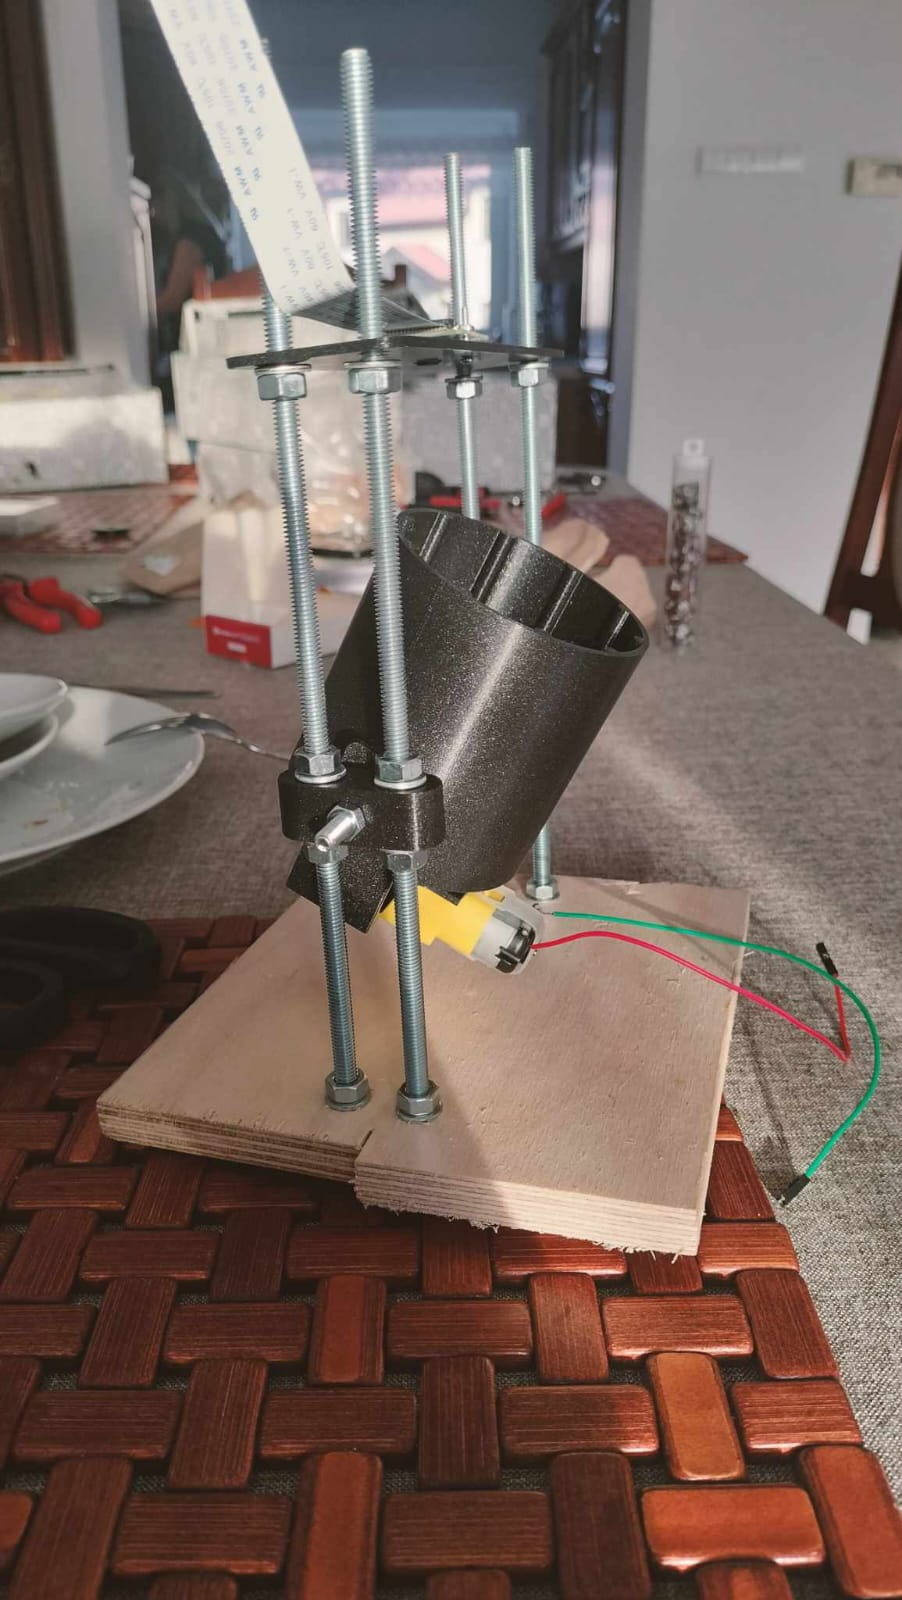
\includegraphics[width=0.25\linewidth, trim={35mm 75mm 35mm 30mm}, clip]{chapters/03-praca-wlasna/figures/pierwszy}
    \caption{\label{fig:pierwszy}Pierwszy prototyp.}
\end{figure}

Do pierwszych testów robota zaprojektowano cztery warianty kształtów kubków. Przy ich projektowaniu wymiary wzorowano na dostępnych tradycyjnych kubkach do gry w kości.
Średnice kubków do gry z reguły są w przedziale 70-90mm.\cite{cup} Przyjęto, że odpowiedni do tego zadania kubek powinien
zawierać pewnego rodzaju nierówności na ściankach. Takie samo założenie przyjęto przy wcześniej wspominanym eksperymencie.\cite{PK} Dzięki temu kostka nie będzie się ślizgać po ściance a zacznie się odbijać od tych nierówności, co 
będzie lepiej imitowało rzut kością wykonany przez człowieka. Z tego powodu z założenia odrzucono tradycyjny model kubka do gry w cylindrycznym kształcie 
o gładkich ściankach. Zaprojektowano cztery wersje kubka (patrz Rys.\ref{fig:kubki}): kubek kwadratowy (nr. 4), kubek sześcienny (nr. 2), kubek sześcienny z dodadkowymi żebrami (nr. 1)
oraz kubek cylindryczny z dodatkowymi żebrami (nr. 3). 
Następnie je przetestowano umieszczając w środku kość do gry i obracając kubek wokół osi przechodzącej przez środek kubka. W czasie testów najgorzej sprawdziły się kubki sześcienne,
ponieważ kości ośmiościenne, które wykorzystywano do testów utykały w narożnikach dociskane przez siłę odśrodkową. Podobny problem pojawiał się przy testach kubka kwadratowego.
Najlepszym wariantem okazał się być cylindryczny kubek z dodatkowymi pionowymi żebrami (nr. 3 na Rys.\ref{fig:kubki}), o które kostka się odbijała podczas kręcenia.
Jego zaletą jest to, że nie posiada on narożników, w których kość mogłaby utknąć. Dodatkowym atutem jest niewielka masa w porównaniu z reszta testowanych wariantów co ma duże znaczenie 
przy obracaniu całego kubka ze względu na moment bezwaładności. \cite{bezwladnosc}

\begin{figure}[H]
    \centering
    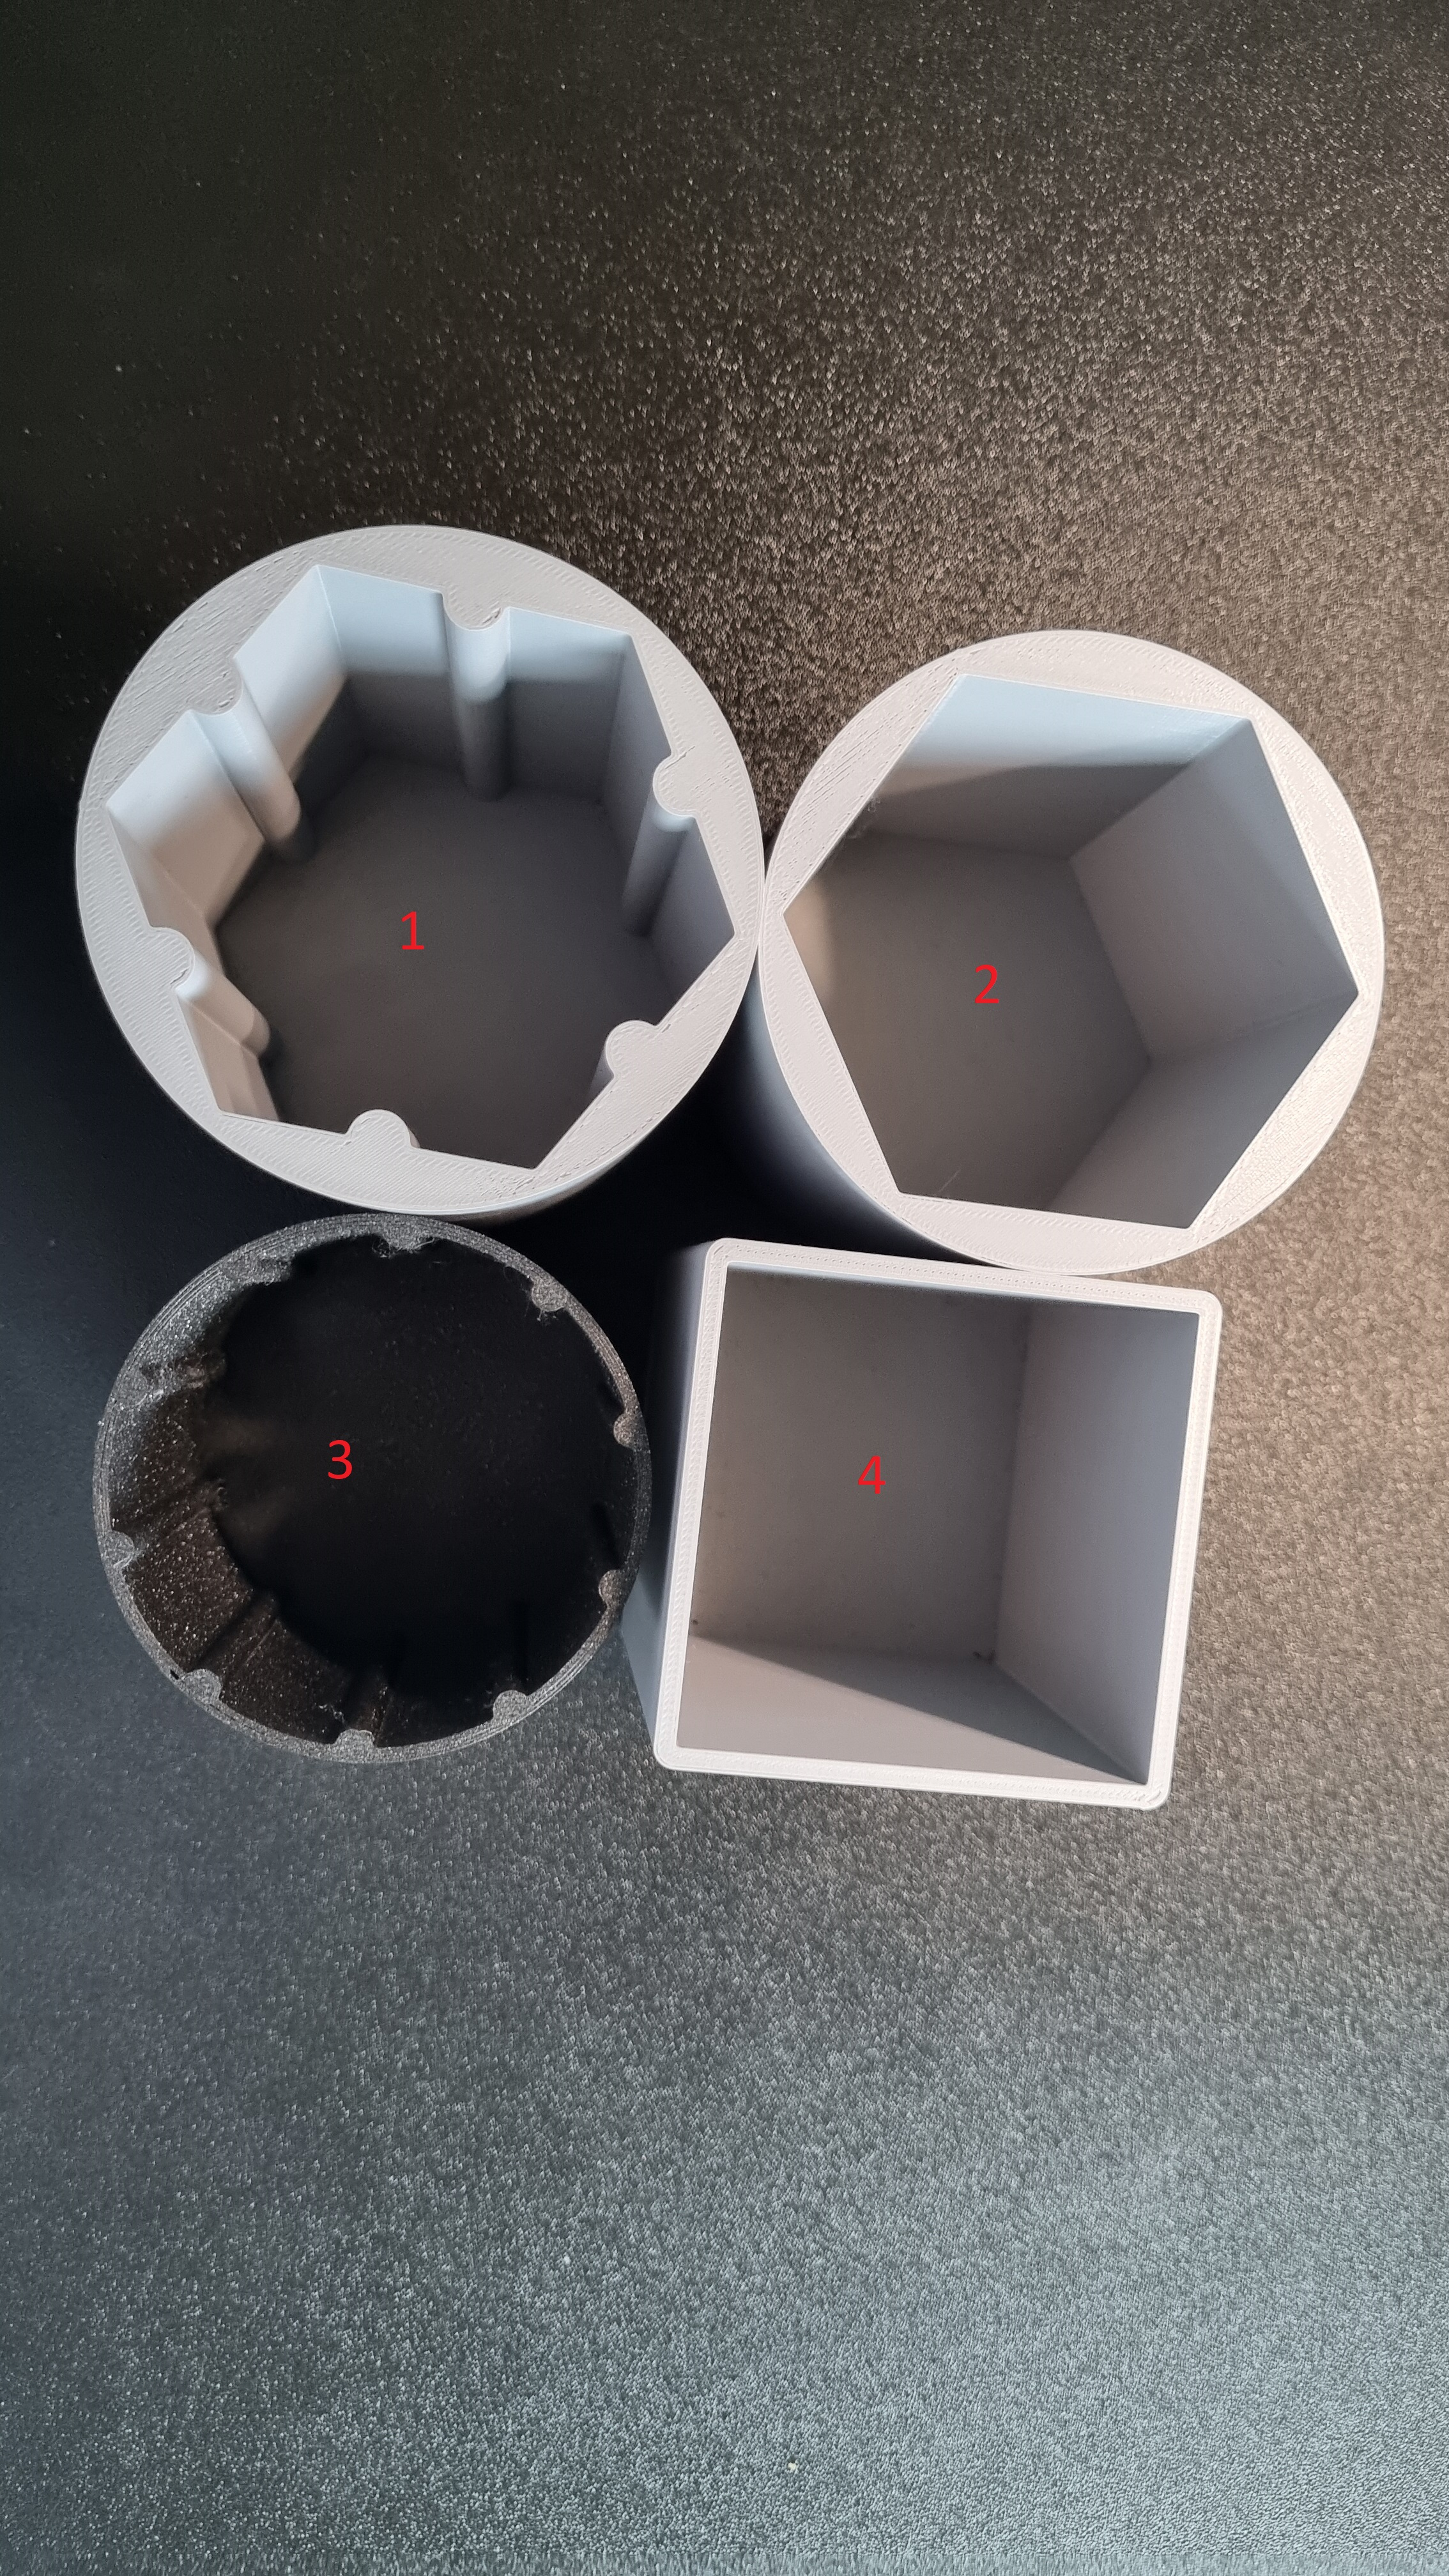
\includegraphics[width=0.65\linewidth, trim={35mm 380mm 20mm 240mm}, clip]{chapters/03-praca-wlasna/figures/kubki.jpg}
    \caption{\label{fig:kubki}Testowane warianty kubków.}
\end{figure}

Po pierwszych testach okazało się, że niezbędny do uzyskania zamierzonego efektu będzie mechanizm, który będzie 
wychylał cały kubek wraz z silnikiem, który odpowiada za jego obrót. Z początku planowano wykorzystanie
serwomechanizmu jednak to rozwiązanie odrzucono, ponieważ większość dostępnych serwomechanizmów, ma
ograniczony obrót do $180^{\circ}$ lub $360^{\circ}$ a to limitowałoby możliwości mechanizmu służącego do wychylania kubka.
Ostatecznie w tym celu wybrano mały silnik krokowy 28BYJ-48, którego moment obrotowy 34,3mNm jest w pełni wystarczający do wychylenia kubka. 
Silnik ten obraca układem dwóch kół zębatych przedstawionych na rysunku \ref{fig:zebatki}.

\begin{figure}[H]
    \centering
    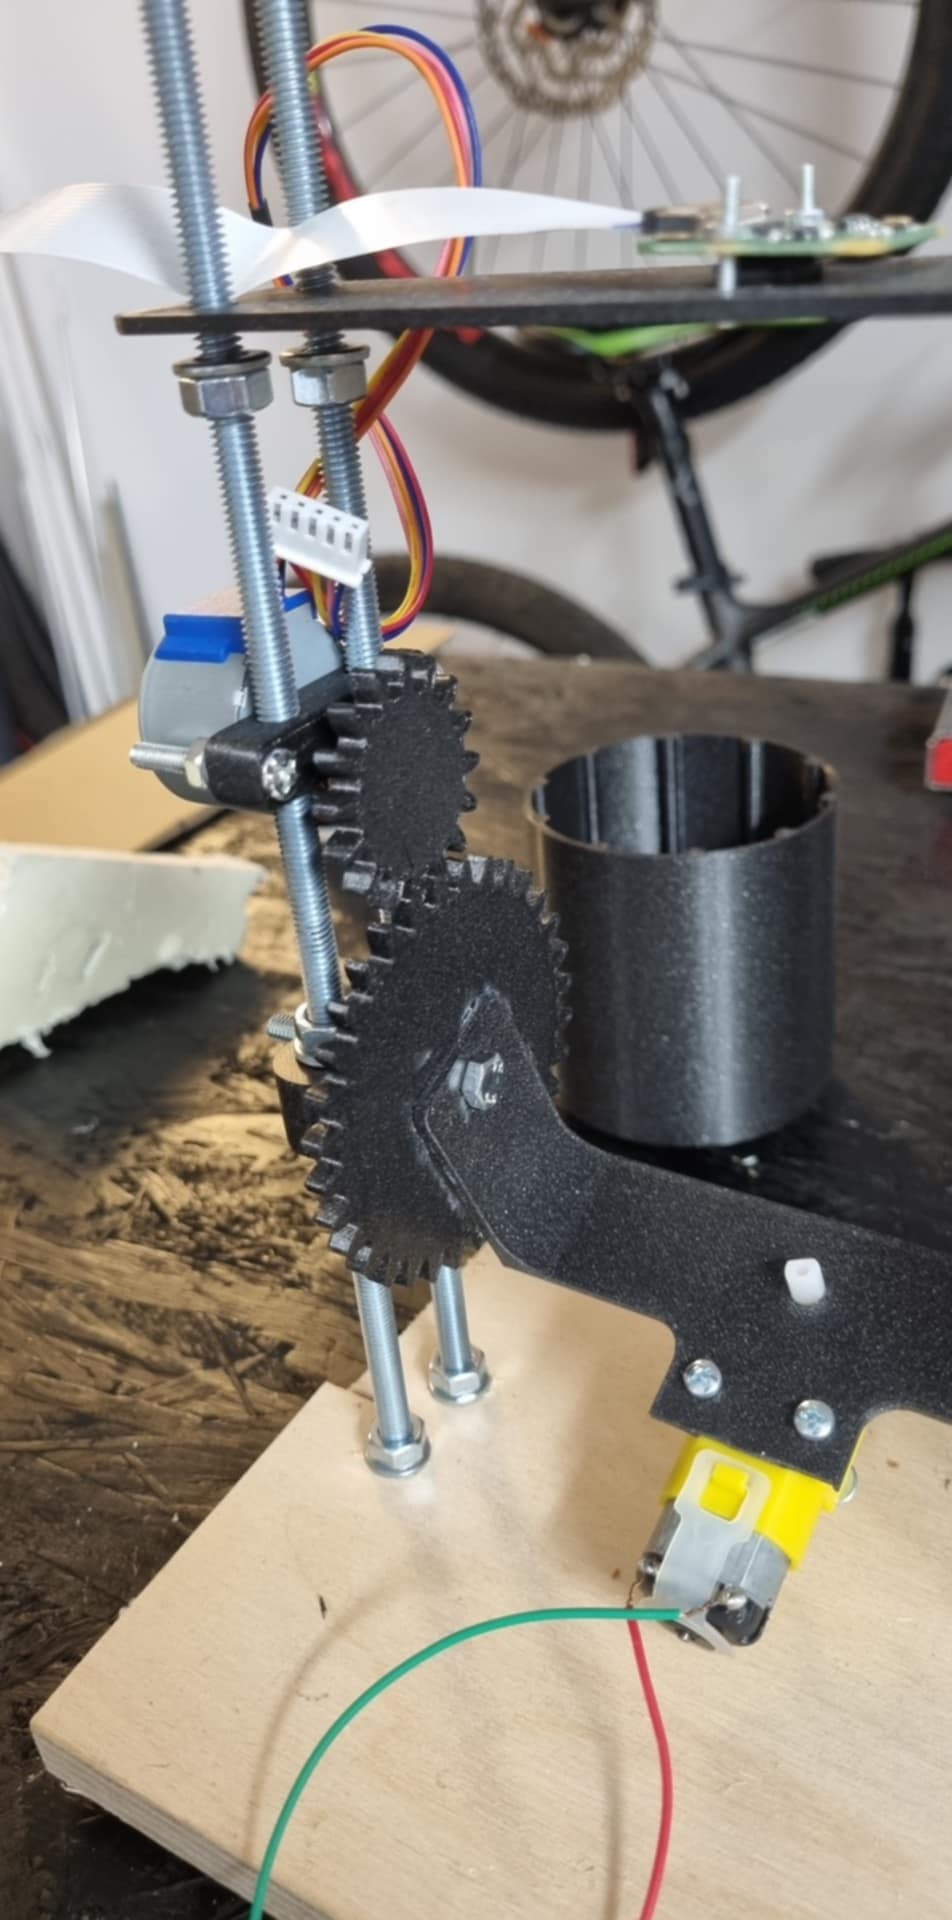
\includegraphics[width=0.25\linewidth, trim={65mm 75mm 0mm 180mm}, clip]{chapters/03-praca-wlasna/figures/koła_zębowe.png}
    \caption{\label{fig:zebatki}Koła zębate.}
\end{figure}

Podczas testów pierwszej wersji robota wykorzytującej obrotowy kubek powstał pomysł alternatywnego rozwiązania.
Rozwiązanie to implementuje inne podejście do rzutu kością. Zamiast obracać cały kubek, a dodatkowo wychylać go,
wykorzystany został trwale zamontowany kubek, na którego dnie znajduje się śmigło, które podcina leżącą na dnie kość.
Takie rozwiązanie znacząco upraszcza cały mechanizm robota oraz bardzo przyspiesza proces losowania liczby. Ten wariant 
nazwano roboczo \textit{blenderem} -- podobnie jak wariant \textit{betoniarki} -- od podobnej zasady działania mechanizmu.

Przy projektowaniu drugiego wariantu robota został wykorzystany ten sam stelaż złożony z metalowych prętów co w 
pierwszym wariancie. Na drukarce 3D wydrukowano dodatkowe części, niezbędne do realizacji tego wariantu.
Zaprojektowano i wydrukowano nowy kubek, śmigło oraz mocowanie dla silnika. Kubek został przystosowany do montażu 
silnika prądu stałego oraz śmigła.

W trakcie testów zauważono, że procesor robota nagrzewa się do wysokich temperatur podczas intensywnej pracy, 
co mogło negatywnie wpływać na jego wydajność i żywotność. Aby temu zapobiec, w projekcie zdecydowano się na 
zastosowanie radiatorów (Rys.\ref{fig:zimno}), które miały pomóc w rozproszeniu nadmiaru ciepła, oraz wentylatora, który 
wspomagał cyrkulację powietrza wokół procesora. Jest to działanie zalecane w oficjalnej dokumentacji na stronie Raspberry Pi, mające przeciwdziałać 
ograniczaniu wydajności w celu ochrony przed przegrzaniem \textit{(Thermal throttling)}.\cite{cooling} 
Dodatkowym problemem wynikającym z rozgrzewania się procesora do wysokich temperatur jest materiał PLA, z którego wykonywane były komponenty robota
oraz prototypów. Materiał ten zaczyna się deformować przy temeraturze $60^{\circ}$C.\cite{plaprusa} Dzięki temu rozwiązaniu udało się obniżyć temperaturę pracy 
procesora, która teraz utrzymuje się w granicach $55^{\circ}$C w czasie rzutów i spada po ich zakończeniu do około $45^{\circ}$C,
co zapewnia stabilne i bezpieczne działanie całego systemu. 
\textcolor{red}{TODO sprawdzic te wartości porównac z włączonym i wyłączonym wentylatorem + dodatkowo sterowanie wentylatorem}

\begin{figure}[H]
    \centering
    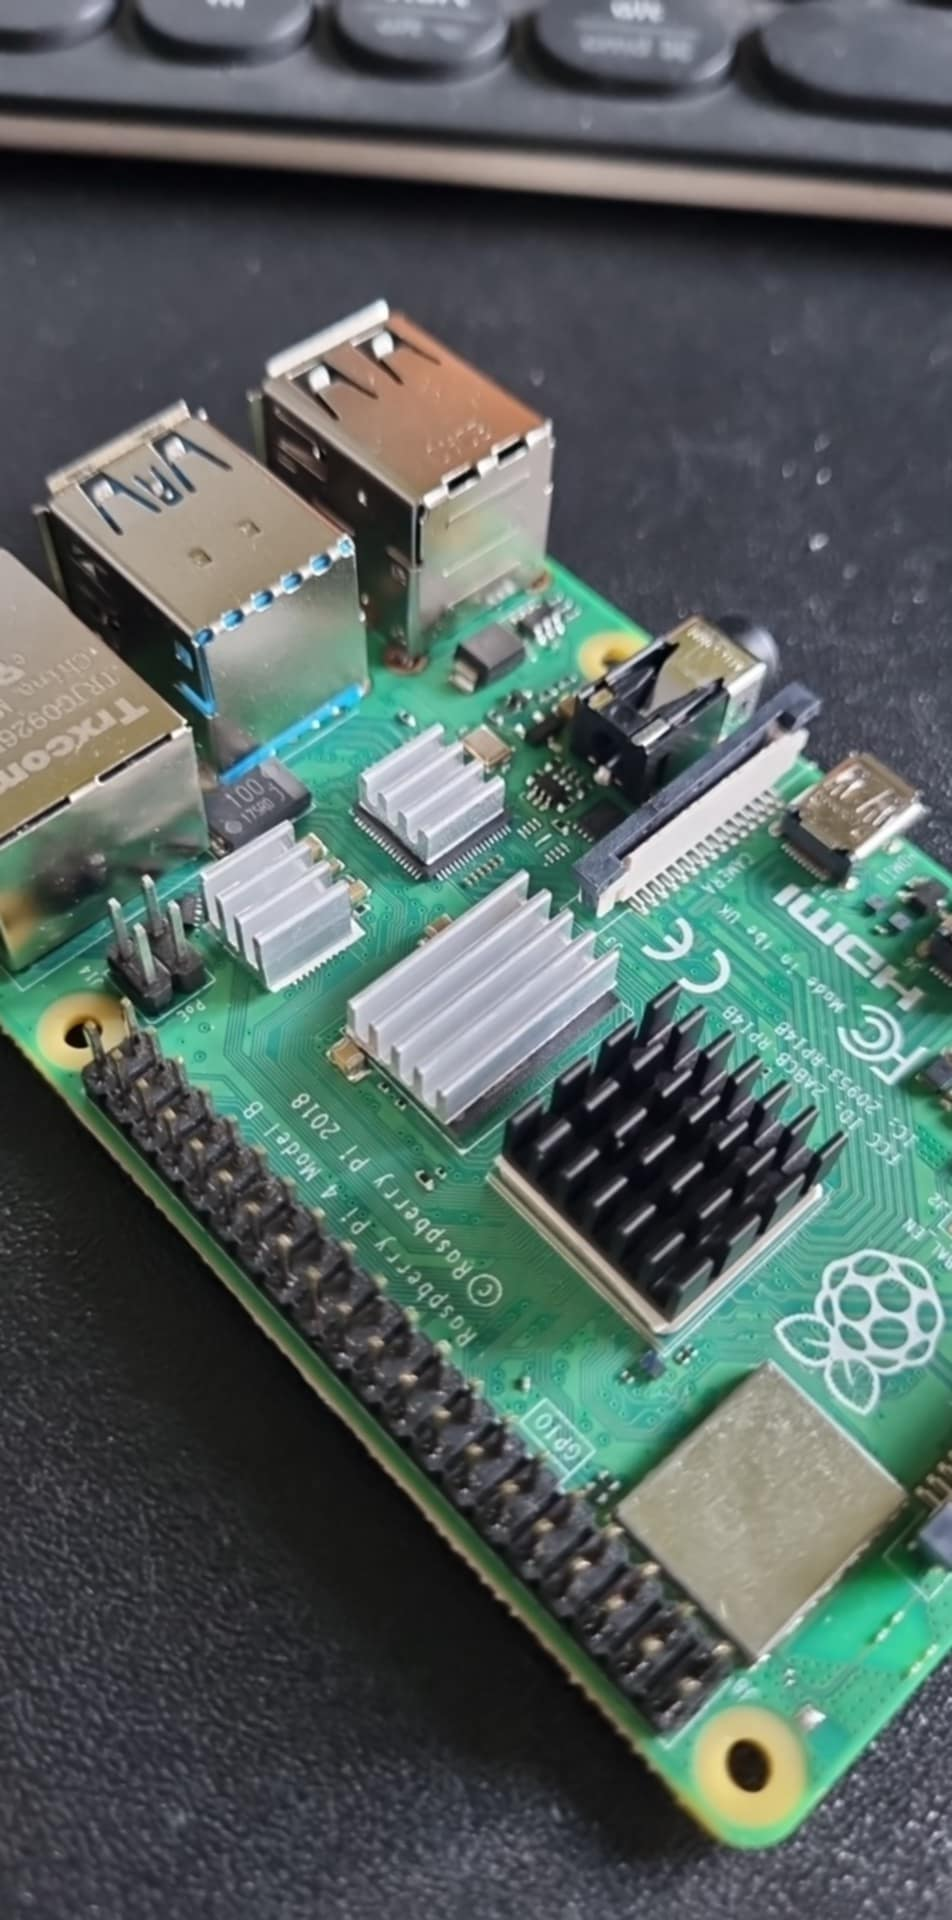
\includegraphics[width=0.25\linewidth, trim={0mm 50mm 0mm 120mm}, clip]{chapters/03-praca-wlasna/figures/now_we_are_cool.png}
    \caption{\label{fig:zimno}Dodane radiatory.}
\end{figure}

Duże znaczenie ma również wykorzystywana kość. Od jej koloru i tekstury zależy jakość zdjęć zrobionych przez
zamonotowaną kamerę. Poniżej przedstawiono dwa przykłady zdjęć i różnic w ich czytelności zależnych od koloru kości.

\begin{figure}[H]
    \centering
    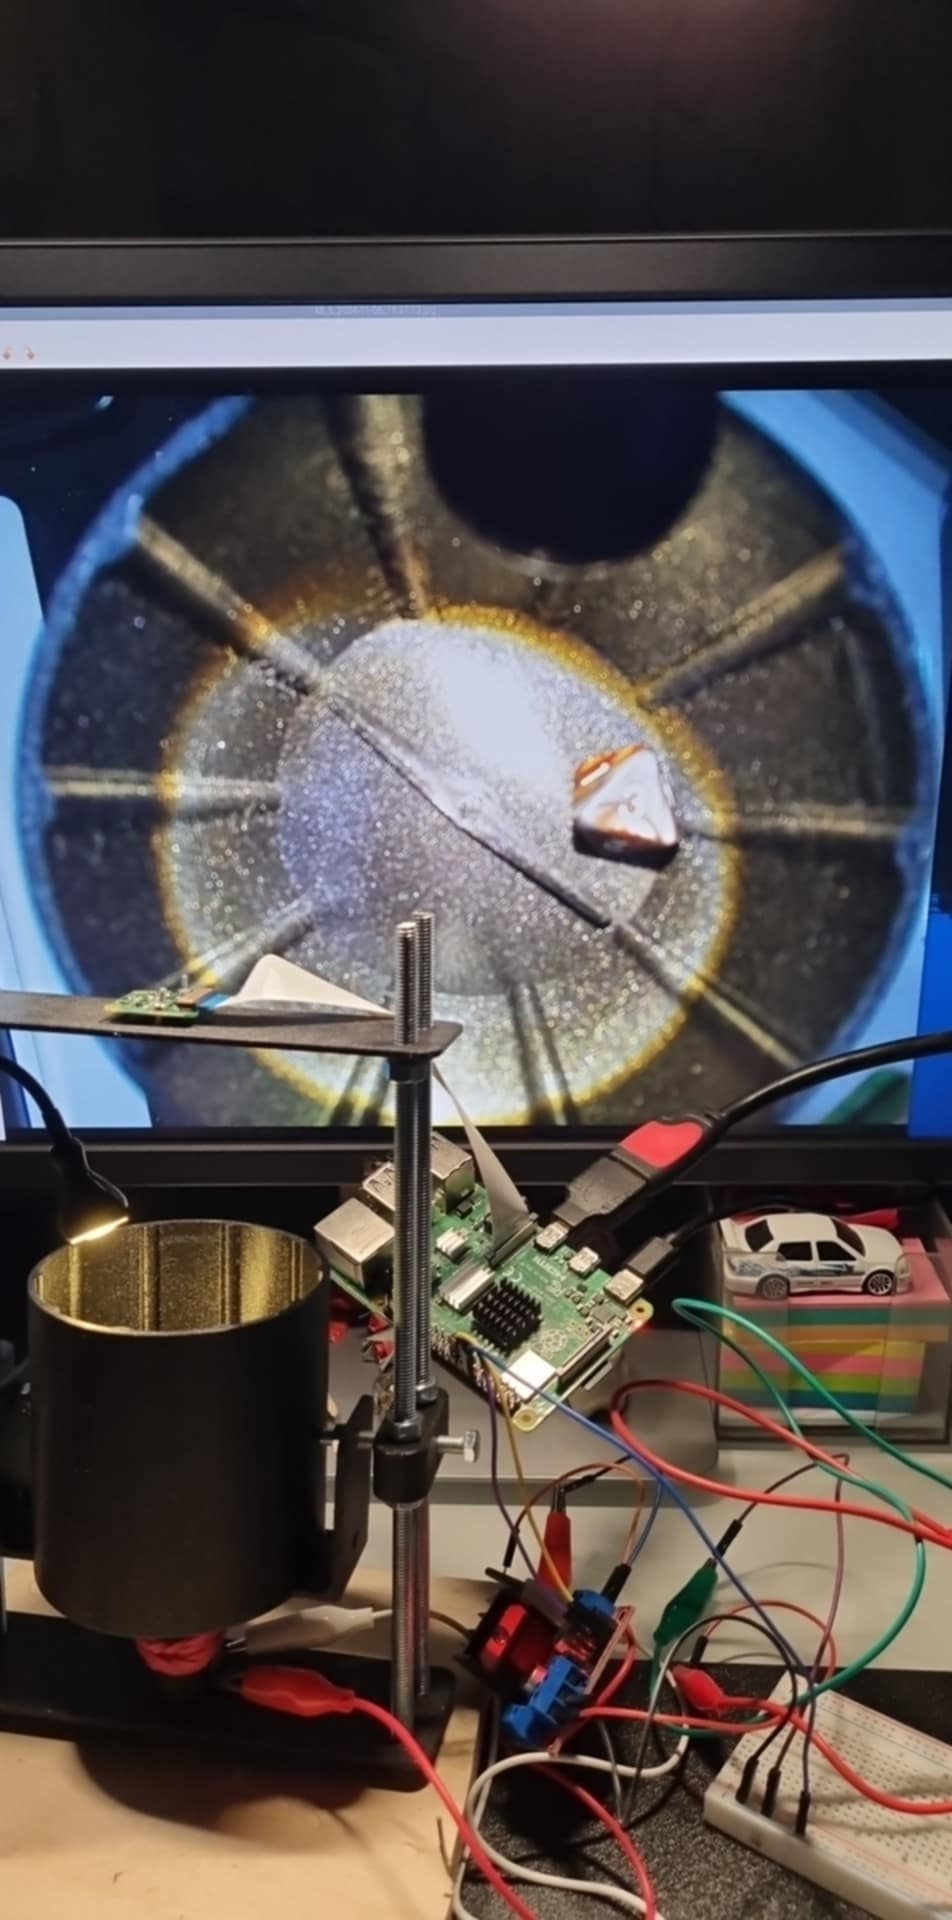
\includegraphics[width=0.25\linewidth, trim={0mm 30mm 0mm 120mm}, clip]{chapters/03-praca-wlasna/figures/nie_widac.png}
    \caption{\label{fig:nie_widac}Kość z teksturą.}
\end{figure}

\begin{figure}[H]
    \centering
    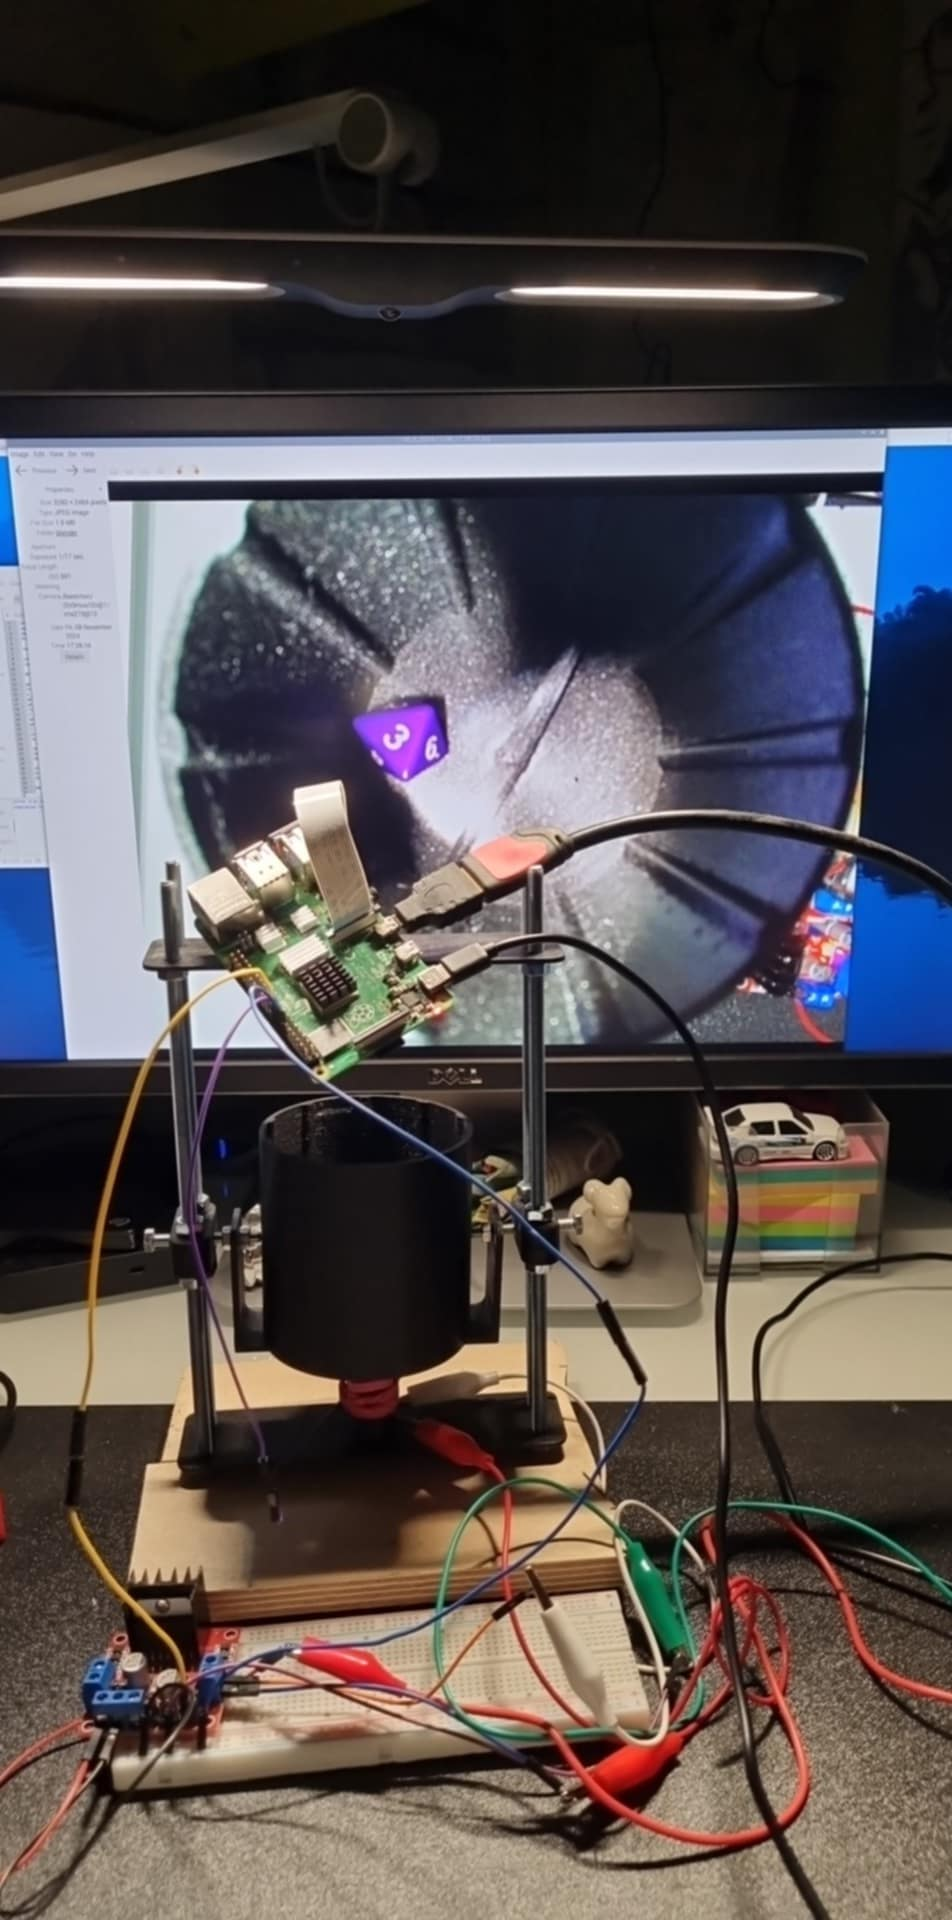
\includegraphics[width=0.25\linewidth, trim={0mm 30mm 0mm 120mm}, clip]{chapters/03-praca-wlasna/figures/widac.png}
    \caption{\label{fig:widac}Jednobarwna kość.}
\end{figure}

W obu wariantach dużym problemem był złej jakości obraz z kamery. W tym celu zaprojektowano system oświetlenia składający się z diod
LED sterowanych przy pomocy układu tranzystorów Darlingtona. Dzięki temu wnętrze kubka stało się dużo jaśniejsze co pozwala kamerze na
robienie zdjęć lepszej jakości. Zdjęcie oświetlonego kubka przedstawiono na Rys.\ref{fig:jasno}. Dodatkowo rozświetlenie wnętrza kubka na tyle poprawiło
jakość zdjęć, że pozwoliło to na obniżenie kamery względem kubka. Spowodowało to że wysokość prototypu zmniejszyła się o około 5cm - 
co było znaczącą poprawą, ponieważ jednym z założeń postawionych na początku budowy było stworzenie urządzenia o niewielkich rozmiarach.
Dzięki tym zabiegom otrzymywane zdjęcia stały się dużo bardziej wyraźne oraz pole widzenia kamery było ograniczone tylko do dna kubka.
Diody LED służące do oświetlenia wnętrza kubka połączono szeregowo. Dzięki temu nie trzeba było wykorzystywać dodatkowych rezystorów a liczba połączeń
jest minimalna, ponieważ wystarczają dwa przewody do podłączenia całego układu diod.

\begin{figure}[H]
    \centering
    \rotatebox{-90}{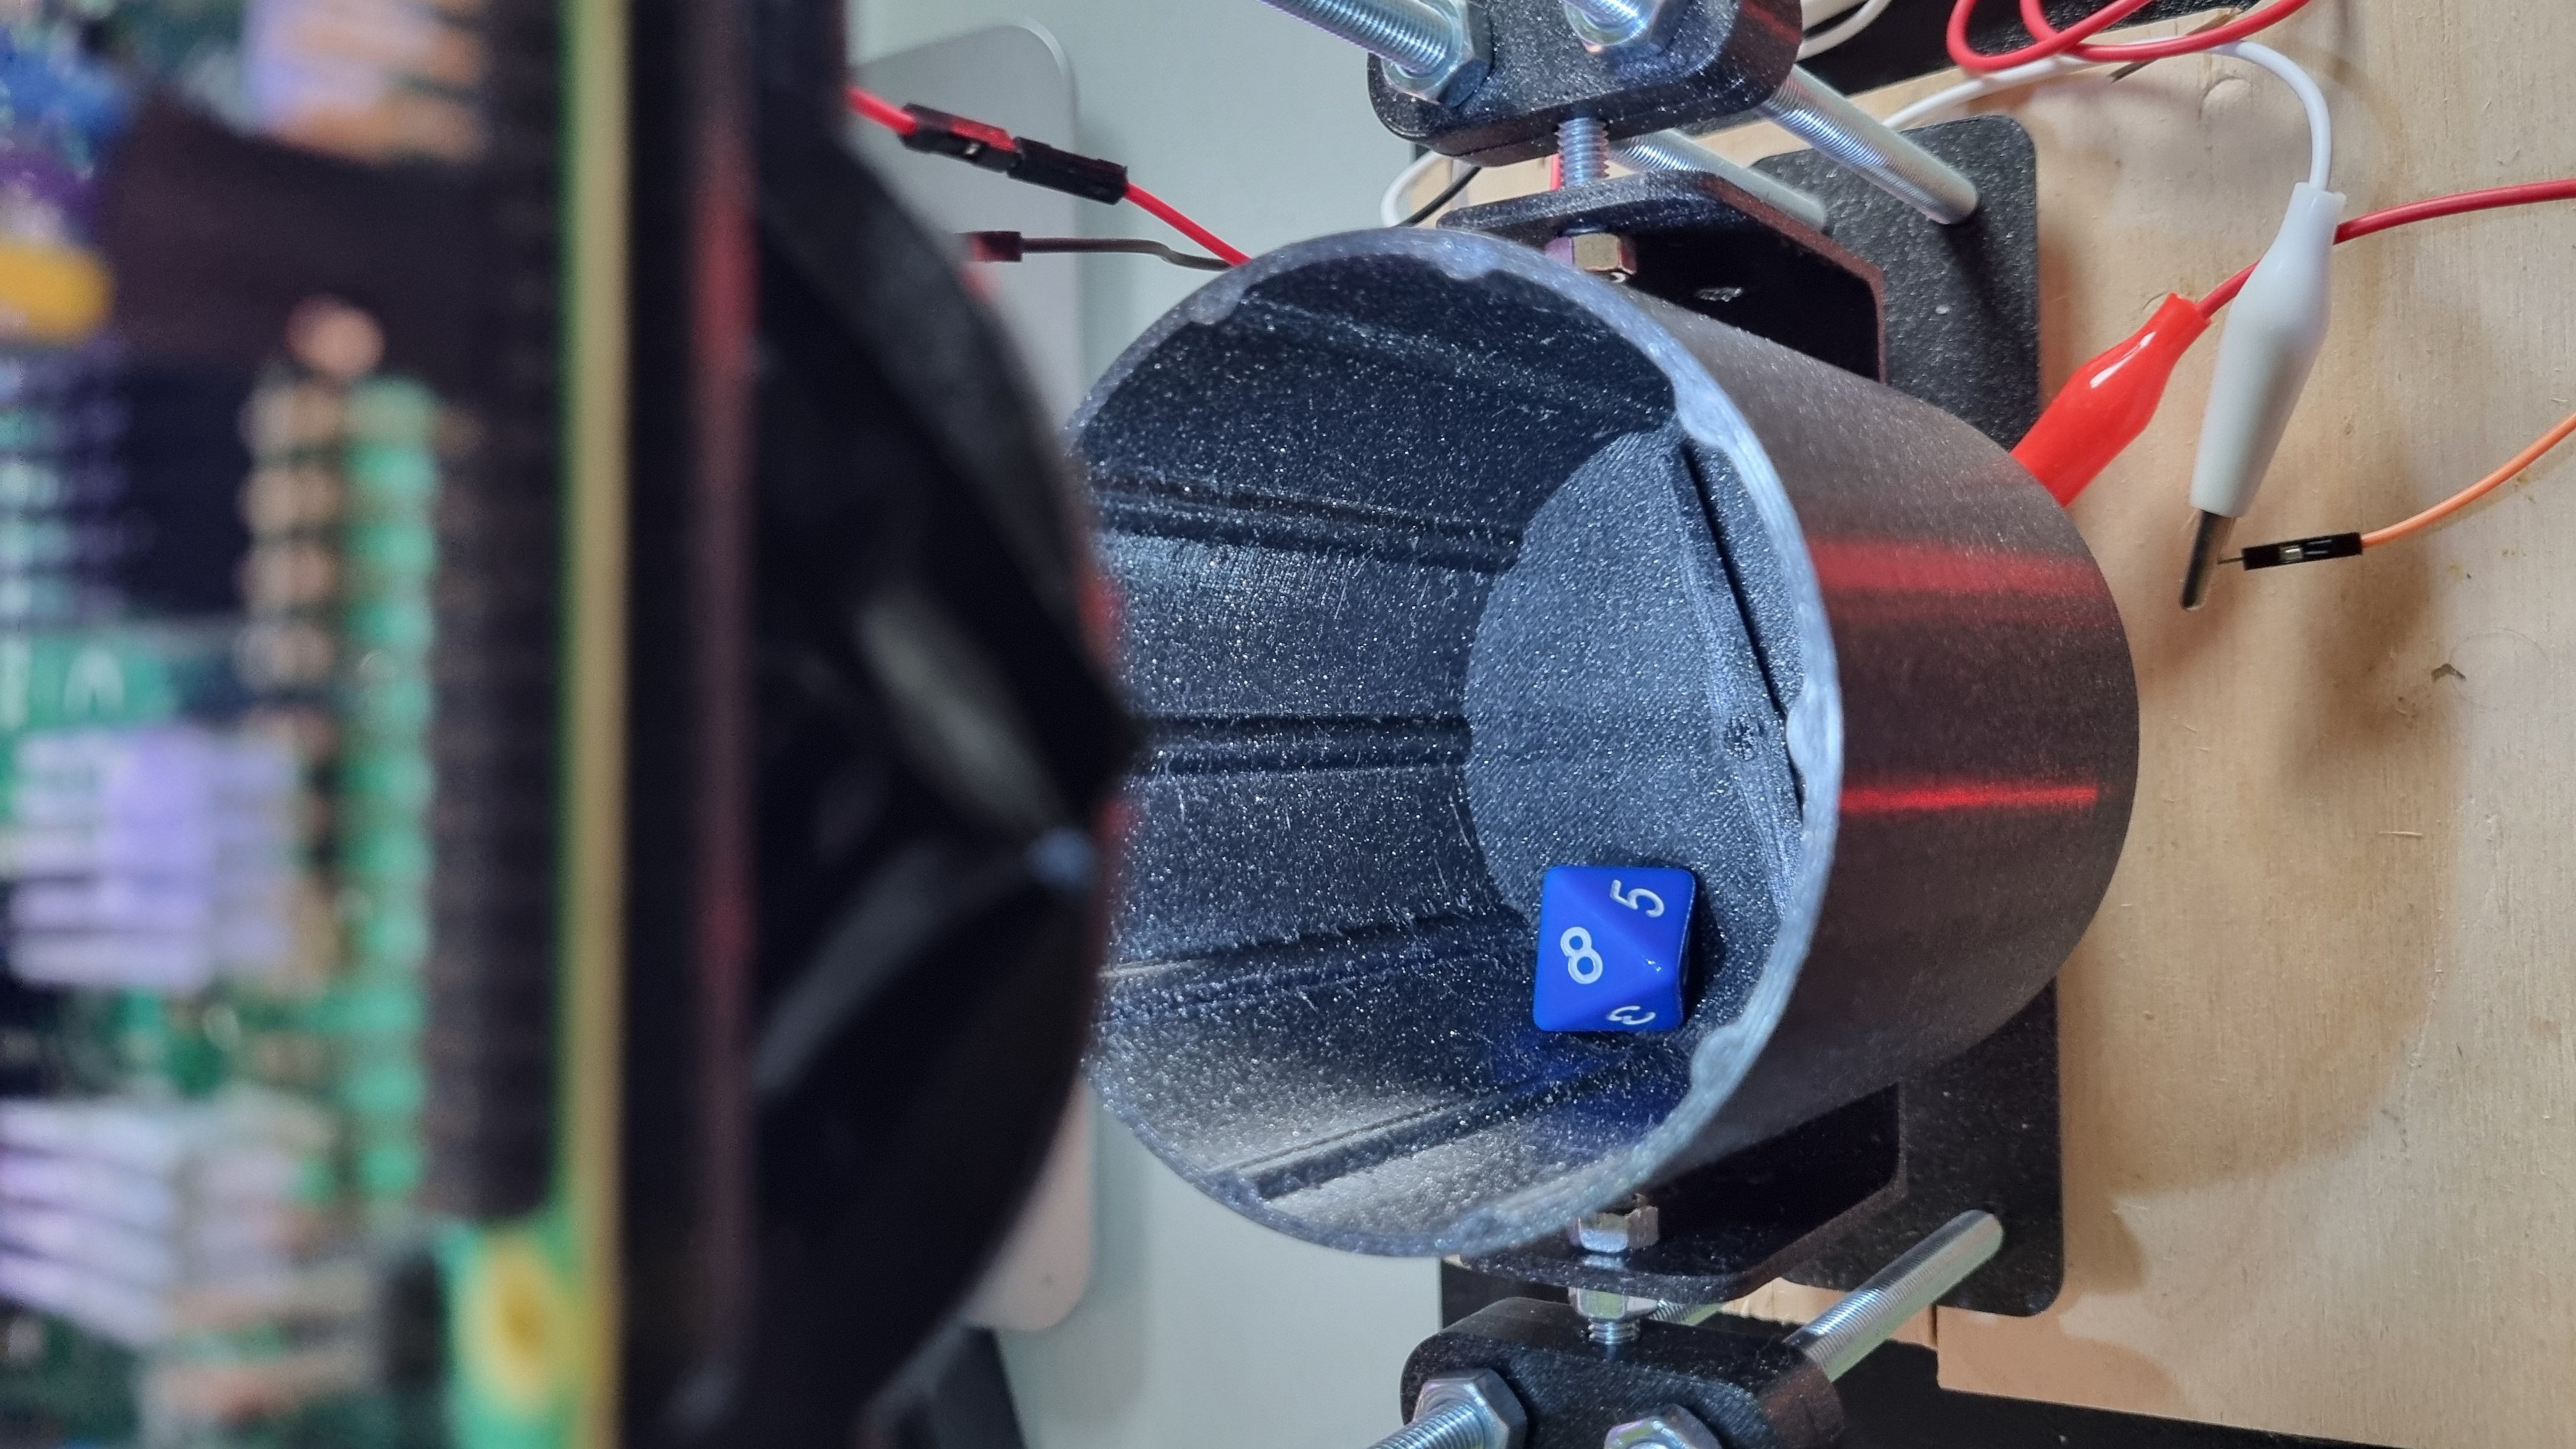
\includegraphics[width=0.45\linewidth]{chapters/03-praca-wlasna/figures/i_stala_sie_jasnosc.jpg}}
    \caption{\label{fig:jasno}Oświetlone wnętrze kubka.}
\end{figure}

Podczas testów prototypów konieczne było również określenie wysokości na której może znajdywać się kamera nad kubkiem. Wysokość tą określono na podstawie 
jakości zdjęć jako najlepszą, podczas testów prototypów. W tym celu wykonano zdjęcia z różną odległością kamery od dna kubka (patrz Rys.\ref{fig:wysoko}-\ref{fig:ideolo}). Głównym celem było znalezienie minimalnej odległości kamery od dna kubka, które nie powodowałoby, 
znacznego pogorszenia się jakości zjęć co utrudniałoby rozpoznawanie wyników na kości. Dodatkową zaletą obniżenia kamery względem kubka był fakt, że kamera 
znajdująca się niżej miała w swoim zasięgu widoku tylko dno kubka co również miało za zadanie ułatwić rozpoznawanie kości oraz jej wartości. W trakcie testowania
odległość tą wyznaczono na 120mm.

\begin{figure}[h]
    \centering
    % Pierwsze zdjęcie
    \begin{minipage}{0.32\textwidth}
        \centering
        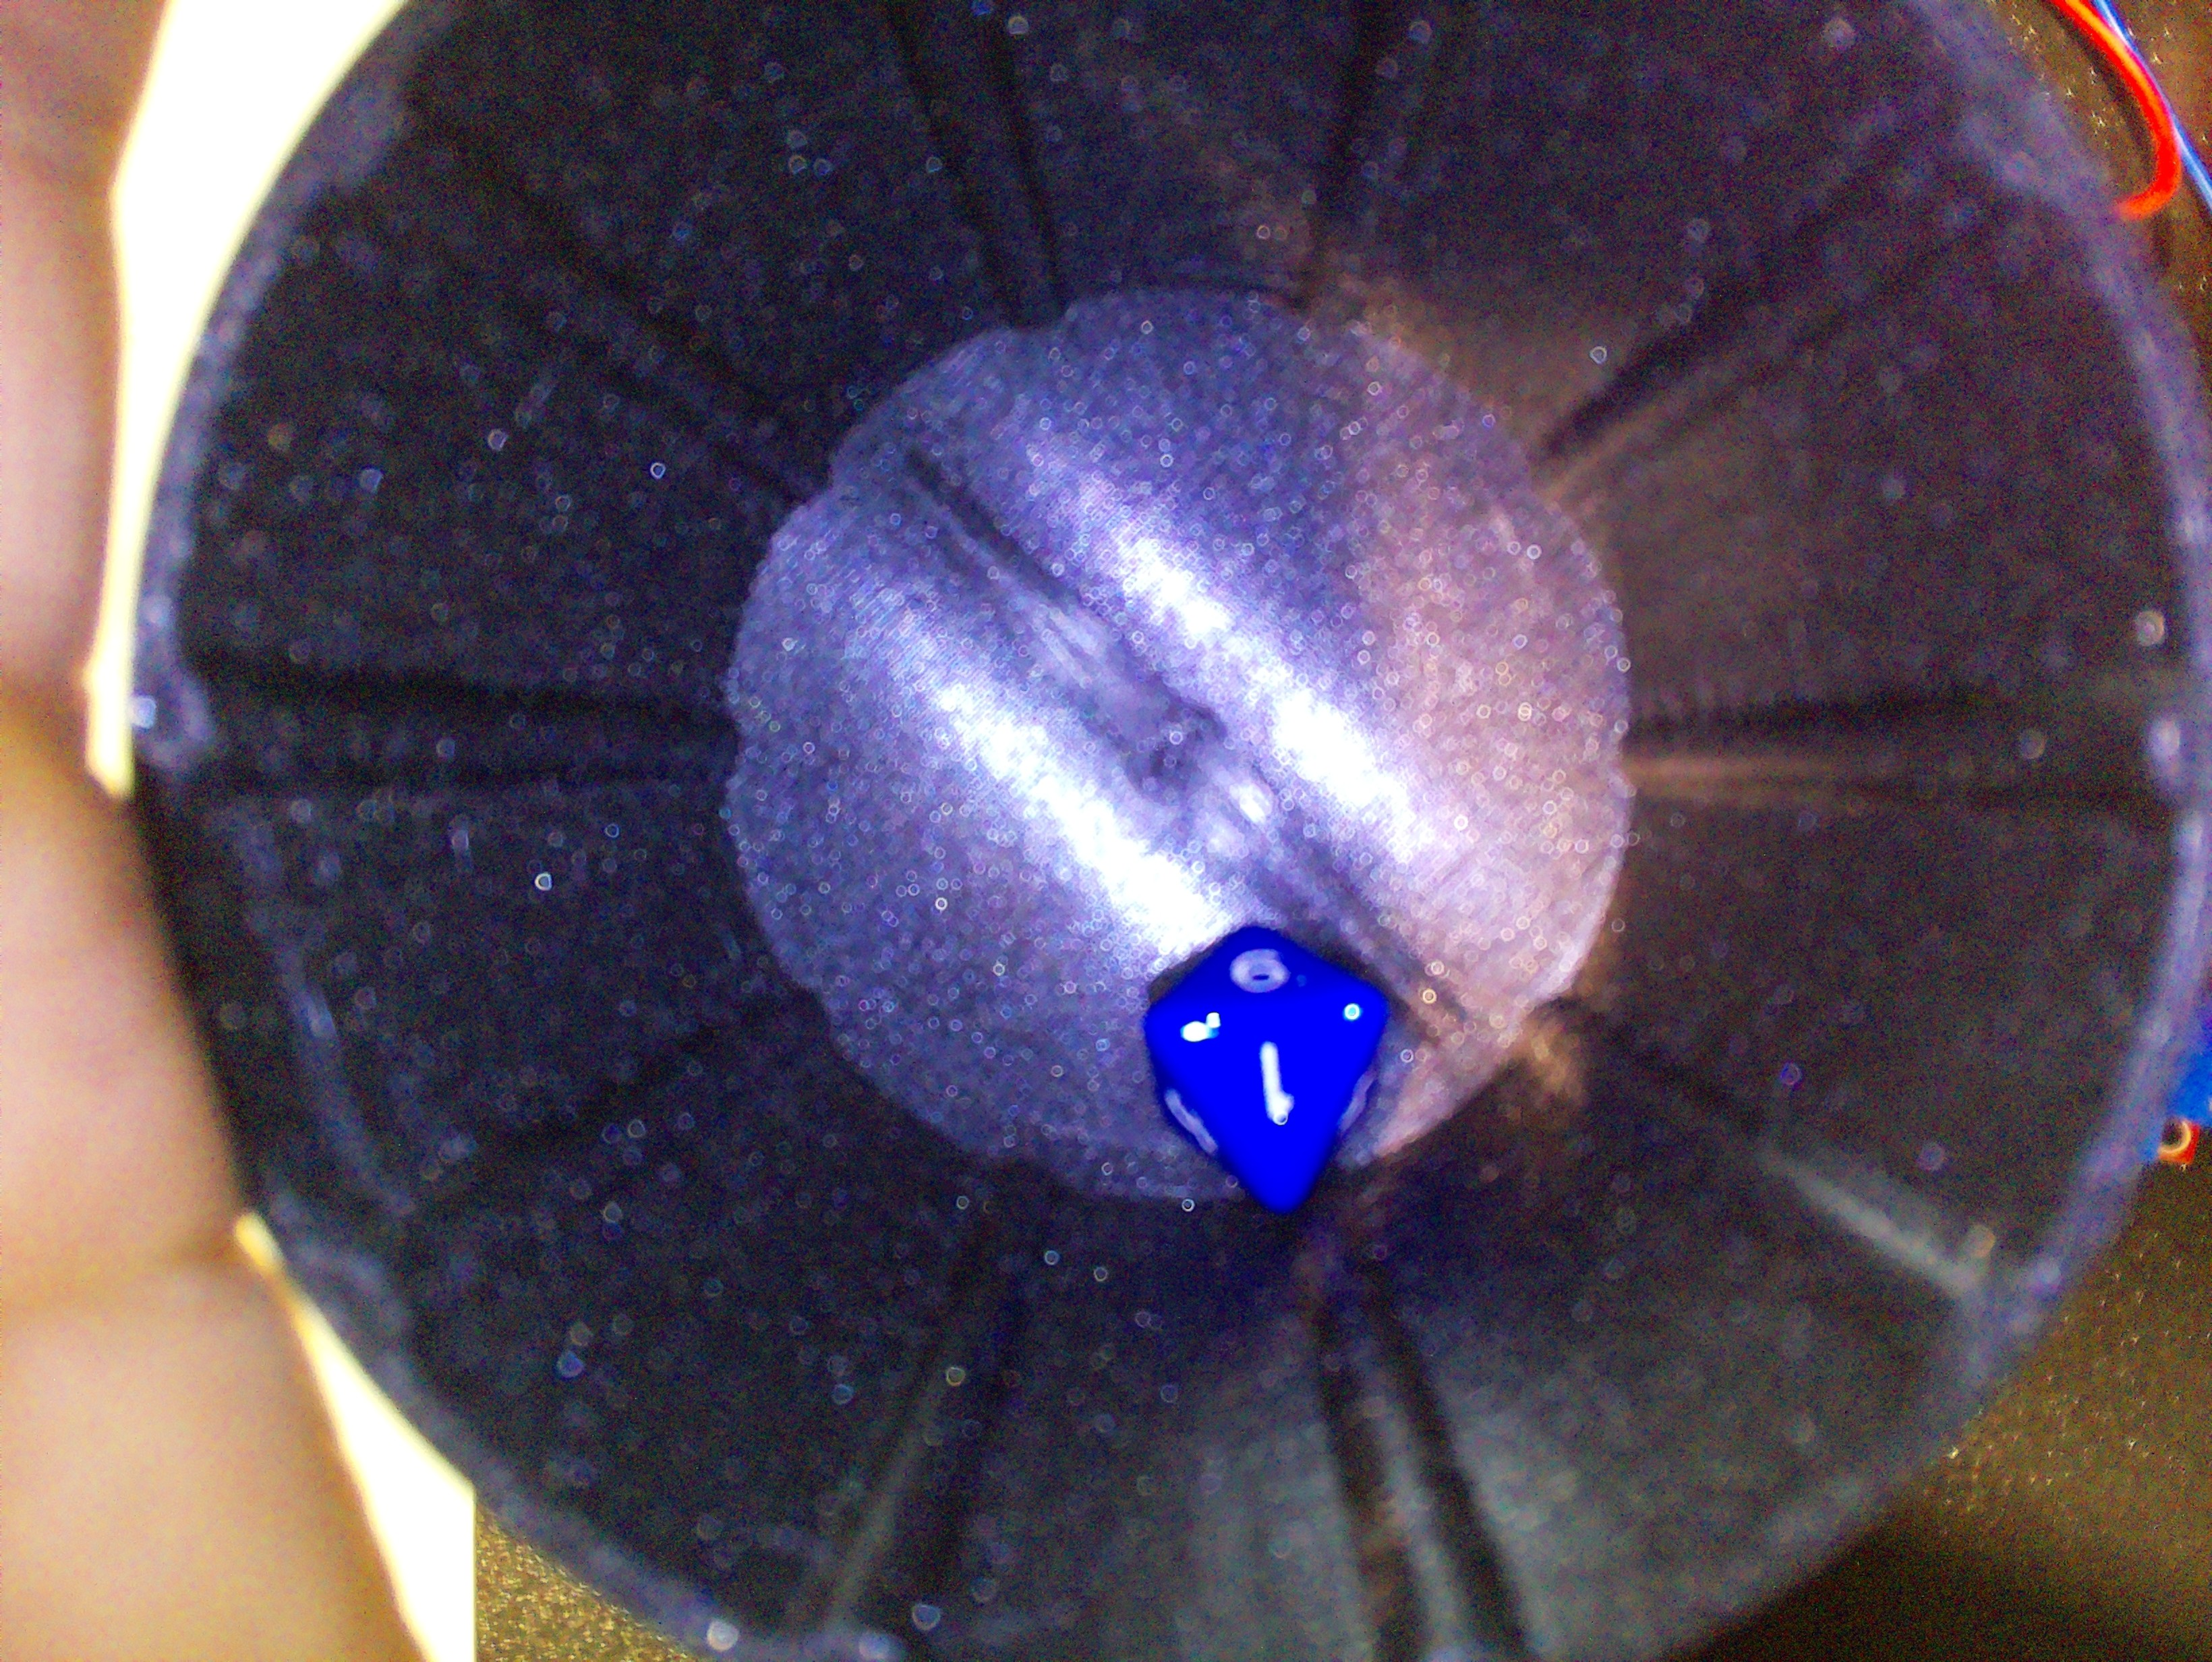
\includegraphics[width=\linewidth]{chapters/03-praca-wlasna/figures/wysoko.jpg}
        \caption{\label{fig:wysoko}Pierwsze ustawienie.}
    \end{minipage}
    \hfill
    % Drugie zdjęcie
    \begin{minipage}{0.32\textwidth}
        \centering
        \includegraphics[width=\linewidth]{chapters/03-praca-wlasna/figures/niżej.jpg}
        \caption{\label{fig:nizej}Drugie ustawienie.}
    \end{minipage}
    \hfill
    % Trzecie zdjęcie
    \begin{minipage}{0.32\textwidth}
        \centering
        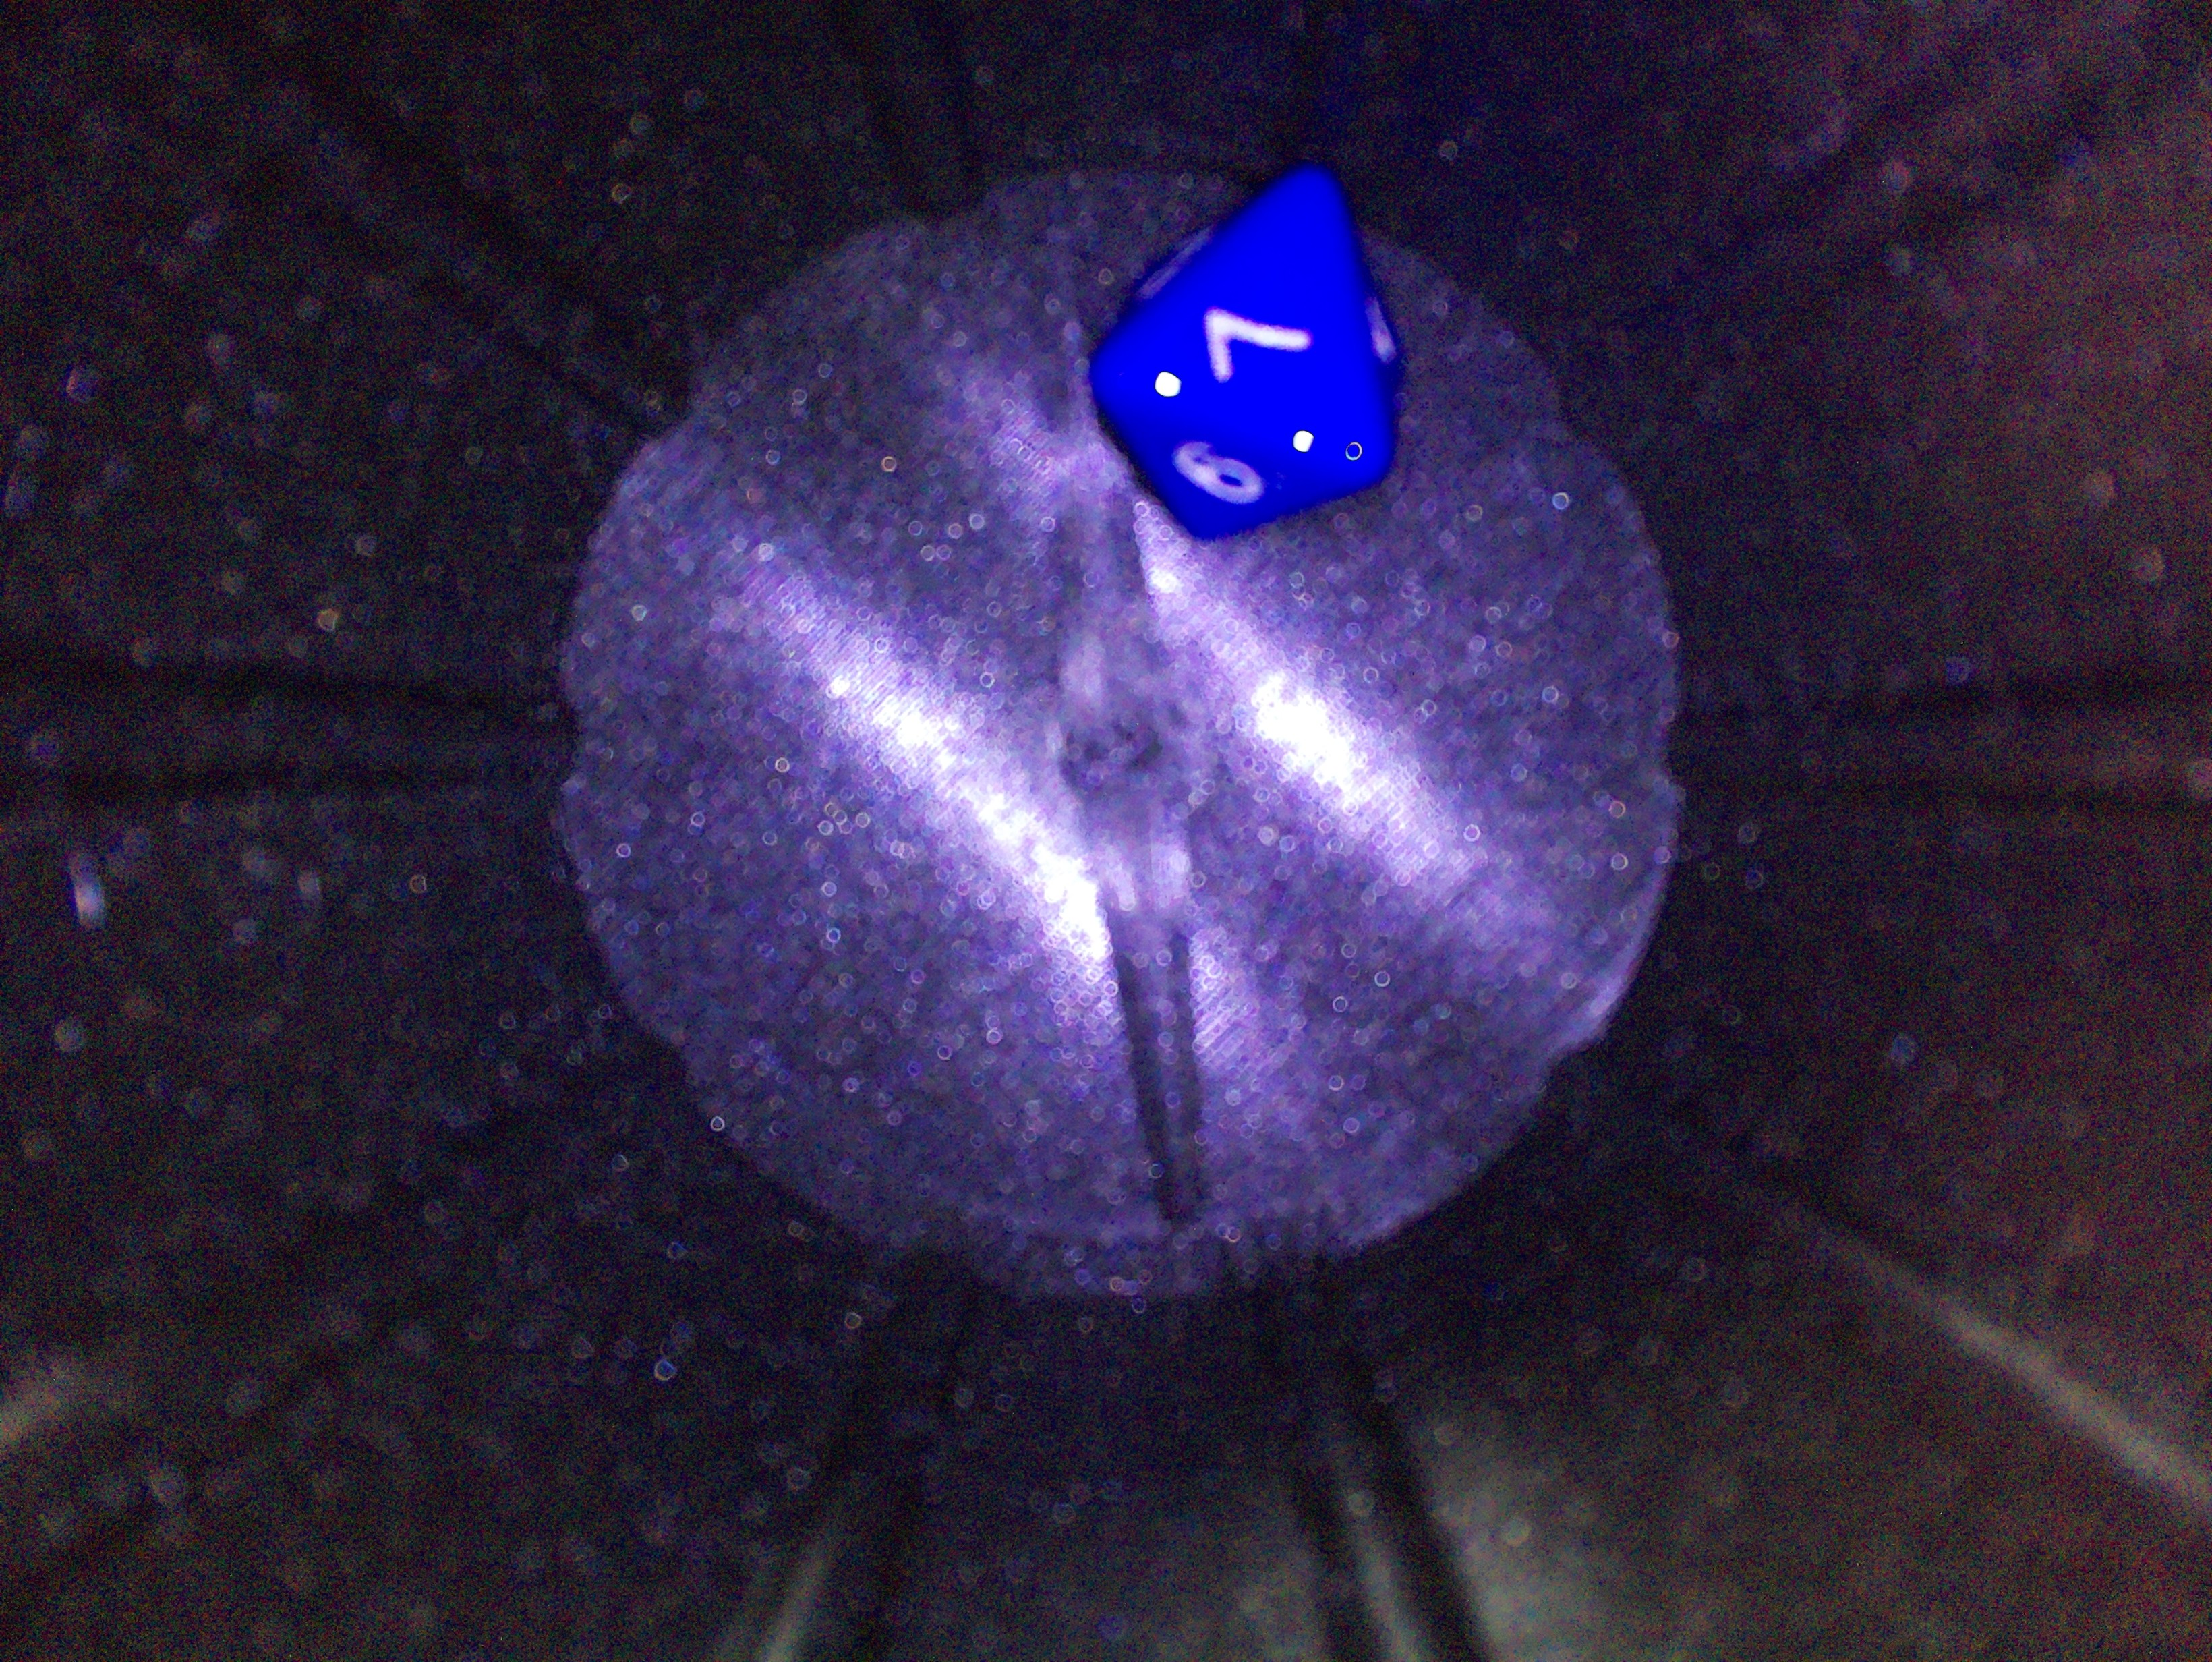
\includegraphics[width=\linewidth]{chapters/03-praca-wlasna/figures/ideolo.jpg}
        \caption{\label{fig:ideolo}Trzecie ustawienie.}
    \end{minipage}
\end{figure}

Po skonstruowaniu obu wersji robota i wstępnym przetestowaniu ich, okazało się, że wariant blendera będzie znacznie szybciej (około 4-krotnie) wykonywał rzut kością.
Pojedyńczy rzut kością za pomocą \textit{bledera} wraz ze zrobieniem zdjęcia trwa około 1,7 sekundy.
Ponadto wersja blendera jest znacznie stabilniejszą konstrukcją, ponieważ nie wymaga poruszania dużymi komponentami robota. 
Największą zaletą wariantu blendera jest prostsza -- w porównaniu z wariantem betoniarki -- budowa spowodowana mniejszą liczbą ruchomych elementów. Jest to ważne z punktu widzenia
długotrwłej eksploatacji podczas, której bardziej skomplikowane mechanizmy szybciej się zużywają. Z tych powodów do docelowego robota wybrano 
wariant blendera. Dzięki temu projekt stał się mniej skomplikowany mechanicznie, a jednocześnie jego użyteczność wzrosła, ponieważ
głównym zadaniem tego robota jest generowanie liczb losowych, a to zadanie szybciej był w stanie wykonywać właśnie ten wariant.

%%%%%%%%%%%%%%%%%%%%%%%%%%%%%%%%%%%%%%%%%%%%%%%%%%%%%%%%%%%%%%%%%%%%%%%%%%%%%%%%%%%%%%%%%%%%%%%%%%%%%%%%%%%%%%%%%%%%%%%%%%%%%%%%%%%%%%%%%%%%%%%%%%%%%%

\subsection{Ostateczna wersja robota}
Projektowanie ostatecznej wersji robota rozpoczęto od przeanalizowania wad, zalet oraz ogólnych cech prototypów. Postanowiono, że komputer oraz układy sterujące będą
umieszczone z boku kubka nie nad tak jak w prototypach, ponieważ sprawiało to, że robot był zbyt wysoki, względem założenia kompaktowego urządzenia.
Na podstawie testów prototypów wywnioskowano, że najlepszym rozwiązaniem będzie zaprojektowanie obudowy umożliwającej łatwy dostęp do wszystkich komponentów.
Postanowiono, że finalna wersja robota będzie wykorzystywała kubek o tej samej średnicy co w prototypie. Oznaczało to, że kubek będzie miał zwenętrzną średnicę 80mm
i ścianki o grubości 2 mm, na których tak jak w protoypie będą pionowe żebra (patrz nr. 3 na Rys.\ref{fig:kubki}). Dookoła kubka, którego ostateczne wymiary wyniosły 126x80mm,
zaprojektowano resztę konstrukcji. Obudowę zaprojektowano w taki sposób żeby była w stanie pomieścić kubek oraz kamerę umieszczoną na wysokości 120mm nad dnem kubka.
Dodatkowo w tylnej oraz dolnej części obudowy pozostawiono przestrzeń na resztę
elementów składowych robota. Wielkość tej przestrzeni wyznaczono poprzez zwymiarowanie pozostałych elementów takich jak silnik, sterownik, wentylator 
czy Raspberry Pi. Te wymiary posłużyły do określenia minimalnej potrzebnej przestrzeni, którą wyznaczono na około 30mm z tyłu, 35mm od dołu oraz 10 od góry kubka. To minimum 
zwiększono w taki sposób, żeby we wnętrzu pomieściły się również przewody i śruby oraz żeby po całkowitym złożeniu pozostała przestrzeń do swobodnego manipulowania
elementami składowymi. \textcolor{red}{TODO wpisywac tu wymiary, odniesienie do dokumentacji robota, odniesienie do dokumentacji elementów?}

Każdy element został zaprojektowany w taki sposób, żeby cały robot był modułowy. Żeby spełnić to założenie, każdy element
zaprojektowano w taki sposób żeby posiadał on specjalne miejsca na inserty lub śruby. Inserty to mosiężne elementy, które za pomocą lutownicy wgrzewa się
w wydruk 3D. Posiadają one wewnętrzny gwint dzięki czemu można do łączenia wydruków wykorzystywać śruby nie uszkadzając samego wydruku przy 
wielokrotnym skręcaniu i rozkręcaniu robota. Dzięki temu założenie modułowości zostało spełnione, ponieważ dzięki śrubom i insertom każdy element robota 
mógł zostać wydrukowany jako osobna część, którą następnie połączono z innymi częściami w prosty do rozłożenia sposób.

\subsubsection{Opis komponentów ostatecznej wersji robota}

Górna część obudowy - pokrywa przedstawiona na Rys.\ref{fig:pokrywa} - mieszcząca kamerę oraz diody LED, została zaprojektowana w taki sposób żeby dostęp do kubka pozostał łatwy. Osiągnięto to
poprzez wykorzystanie prostego mocowania pokrywy do obudowy, z wykorzystaniem pojedyńczej śruby oraz magnesów neodymowych. Dzięki temu w przypadku kiedy konieczny 
jest dostęp do kamery lub diod LED wystarczy zdjąć tylną scianę robota oraz odkręcić pojedyńczą śrubę. Dodatkowo magnesy neodymowe zapewniają
dobre przyleganie pokrywy do reszty obudowy. Ich dodatkową zaletą jest blokowanie pokrywy w ustalonej pozycji podczas umieszczania kości wewnątrz
kubka.

\begin{figure}[H]
    \centering
    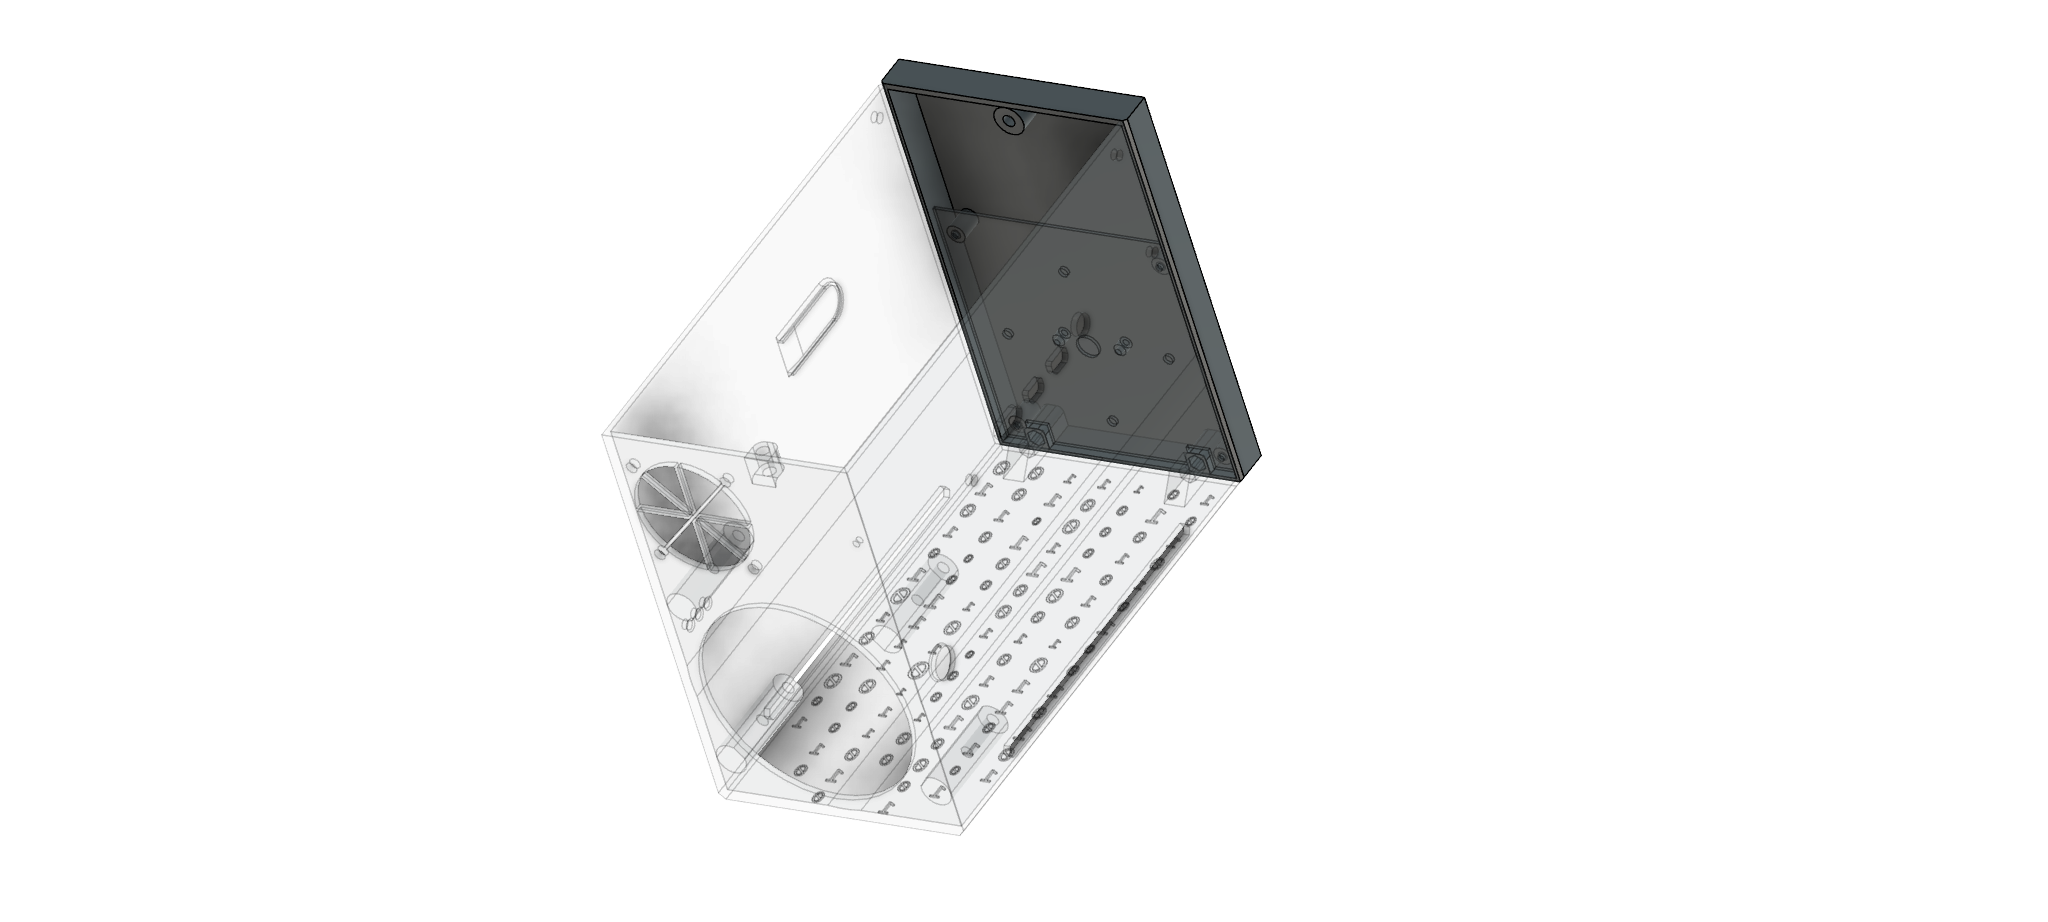
\includegraphics[width=0.95\linewidth]{chapters/03-praca-wlasna/figures/pokrywa.png}
    \caption{\label{fig:pokrywa}Pokrywa obudowy.}
\end{figure}

Dla zapewnienia sztywności całej konstrukcji oraz punktu mocowania dla tylniej ściany robota zaprojektowano belkę przykręcaną do obu ścian. W tą belkę -- przedstawioną na Rys.\ref{fig:belka} --
wkręcana jest również wcześniej wspominana śruba mocująca pokrywę obudowy.

\begin{figure}[H]
    \centering
    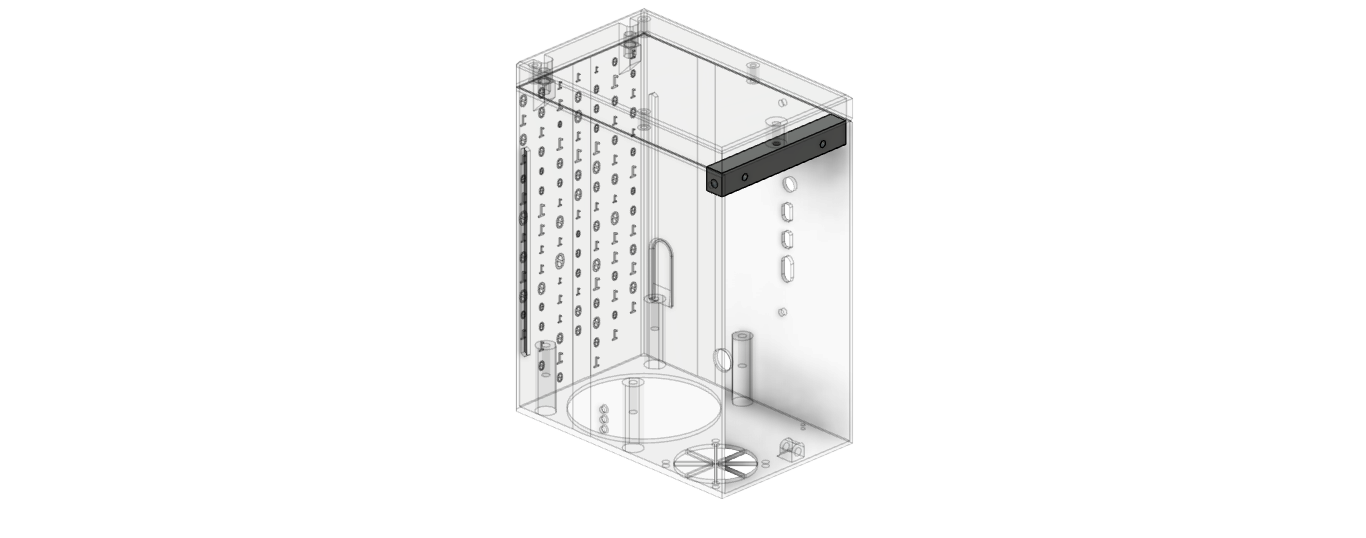
\includegraphics[width=0.95\linewidth]{chapters/03-praca-wlasna/figures/belka.png}
    \caption{\label{fig:belka}Belka.}
\end{figure}

Kamera wraz z diodami LED służącymi do oświetlenia wnętrza kubka znajdujde się w pokrywie. Kamerę zamontowano przy użyciu dwóch śrub M2 natomiast
diody LED umieszczono w zaprojektowanych w wydruku otworach.

W pokrywie znajdują się również dwa sześciokątne otwory na magnesy neodymowe. Dzięki temu że otwory są sześciokątne to walcowe magnesy idealnie
się w nie wpasowują i po wciśnięciu nie wypadają. W drugiej części obudowy znajdują się takie same otwory na drugą parę magnesów. Dla pewności podczas umieszczania magnesów 
wykorzystano klej cyjanoakrylowy.

Kubek, w którym dokonywane są rzuty kością, zaprojektowano na podstawie kubka z prototypowej wersji blendera. Zachowano jego średnicę oraz kształt i rozmieszczenie wewnętrznych
żeber. Zmieniona została zasada mocowania kubka w taki sposób, żeby był on przystosowany do zamocowania w obudowie. W tym celu zaprojektowano
cztery mocowania widoczne na Rys.\ref{fig:kubek}, znajdujące się u dołu kubka, za pomocą których kubek jest przykręcany do obudowy. Dodatkowo pogrubiono dno kubka tak żeby można było w nim umieścić inserty służące 
do przykręcenia uchwytu silnika. Ostatnią modyfikacją było podwyższenie kubka w taki sposób, żeby wysokością sięgał on aż do mocowania kamery - górnej pokrywy.
Dzięki temu podczas rzutów zniknął problem z wypadającą kością, co było dość częstym zajwiskiem podczas testów prototypu. Niestety takie rozwiązanie
spowodowało, że wnętrze kubka przestało być widoczne z zewnątrz. Jednak uznano, że widok z zewnątrz na wnętrze kubka nie jest konieczny do osiągnięcia celów projektu.

\begin{figure}[H]
    \centering
    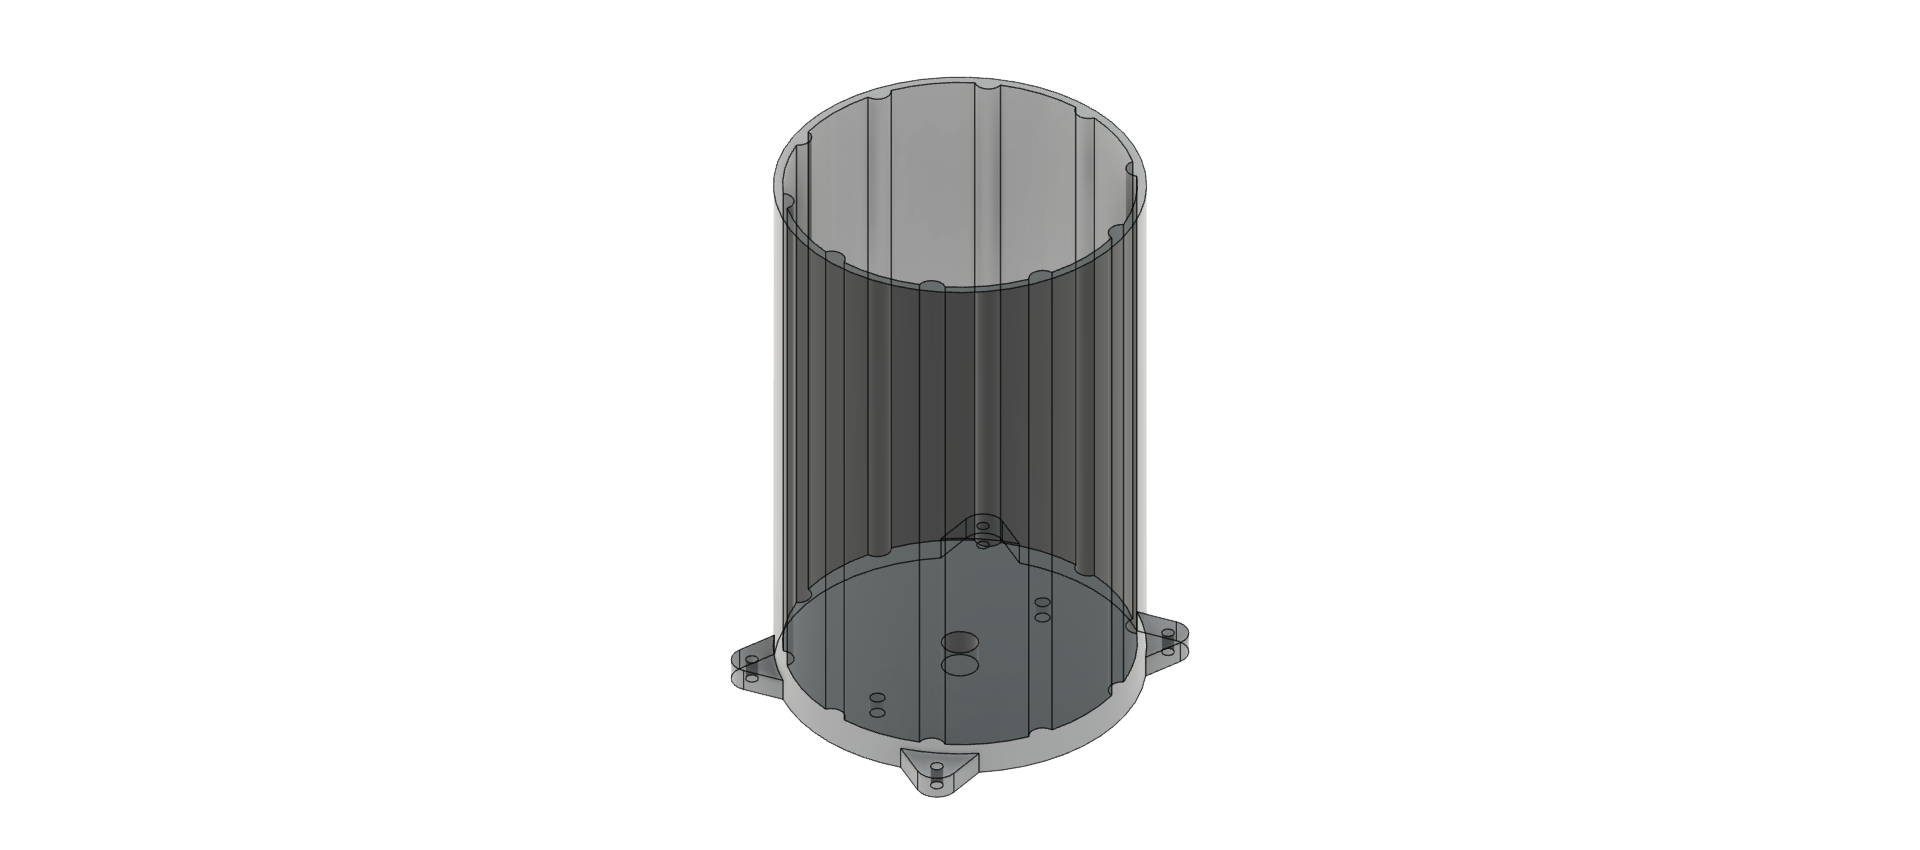
\includegraphics[width=0.95\linewidth]{chapters/03-praca-wlasna/figures/kubek.png}
    \caption{\label{fig:kubek}Kubek.}
\end{figure}

Projekt pierwszego uchwytu mocującego silnik składał się z miejsca do umieszczenia silnika oraz dwóch cylindrycznych słupków służących za prowadnice
śrub mocujących cały uchwyt do dna kubka. Jednak, ponieważ podczas testów pojawiły się problemy z pierwszym silnikiem i wymieniono go na inny, konieczne
było zaprojektowanie drugiego uchwytu. Podczas projektowania drugiego uchwytu wzorowano sie na projekcie pierwszego, jednak dodano dodatkowy trzeci
cylindryczny słupek na śrubę, która miała służyć do kontrolowania wychylenia całego uchwytu w osi przód-tył. Zwiększyło to możliwość regulacji i w ten sposób
ograniczono tarcie śmigla o dno kubka. 

Śmigło zaprojektowano w taki sposób żeby obracając się przy samym dnie kubka, po uderzeniu w kość, wybijało ją w górę. Ten efekt uzyskano
dzięki niskiemu profilowi śmigła oraz bocznych ścian śmigła nachylonych pod kątem $45^{\circ}$.

Podczas testów ostatecznej wersji robota napotkano wcześniej wspominane problemy z pierwotnie wykorzystywanym silnikiem DC 6V. Silnik ten miał okrągły wał przez co śmigło musiało
być bardzo dokładnie spasowane aby uniknąć ślizgania się wału wewnątrz otworu śmigła. To sprawiało, że montowanie śmigła i jego demontaż był bardzo trudny. Dodatkowo po wielokrotnych rzutach kością, śmigło
wbijało się coraz niżej na wał silnika i w ostateczności tarło o dno kubka tak mocno, że silnik nie był w stanie się obracać. 
Żeby temu zaradzić umieszczono pomiędzy śmigłem a dnem kubka metalową podkłądkę, po której śmigło mogło się ślizgać łatwiej niż po dnie kubka. To
jednak nie rozwiązało problemu ponieważ po kolejnych kilku tysiącach rzutów śmigło zaczęło się blokować. 
Z tego powodu postanowiono wymienić silnik na mocniejszy 12V silnik z przekładnią, który ma mniejszą częstotliowść obrotu (około 2000RPM zamiast 4000RPM) ale ma większy moment obrotowy.
Zaletą nowego silnika jest jego wał w kształcie litery "D". Pozwala to na znacznie luźniejsze spasowanie otworu śmigła z wałem przez co 
demontaż śmigła jest znacznie łatwiejszy. Ponadto nowy silnik jest znacznie cichszy niż poprzedni. Obie wersje uchwytów silnika przedstawiono na Rys.\ref{fig:uchwyt_v1} oraz Rys.\ref{fig:uchwyt_v2}.

\begin{figure}[H]
    \centering
    \begin{minipage}{0.48\textwidth}
        \centering
        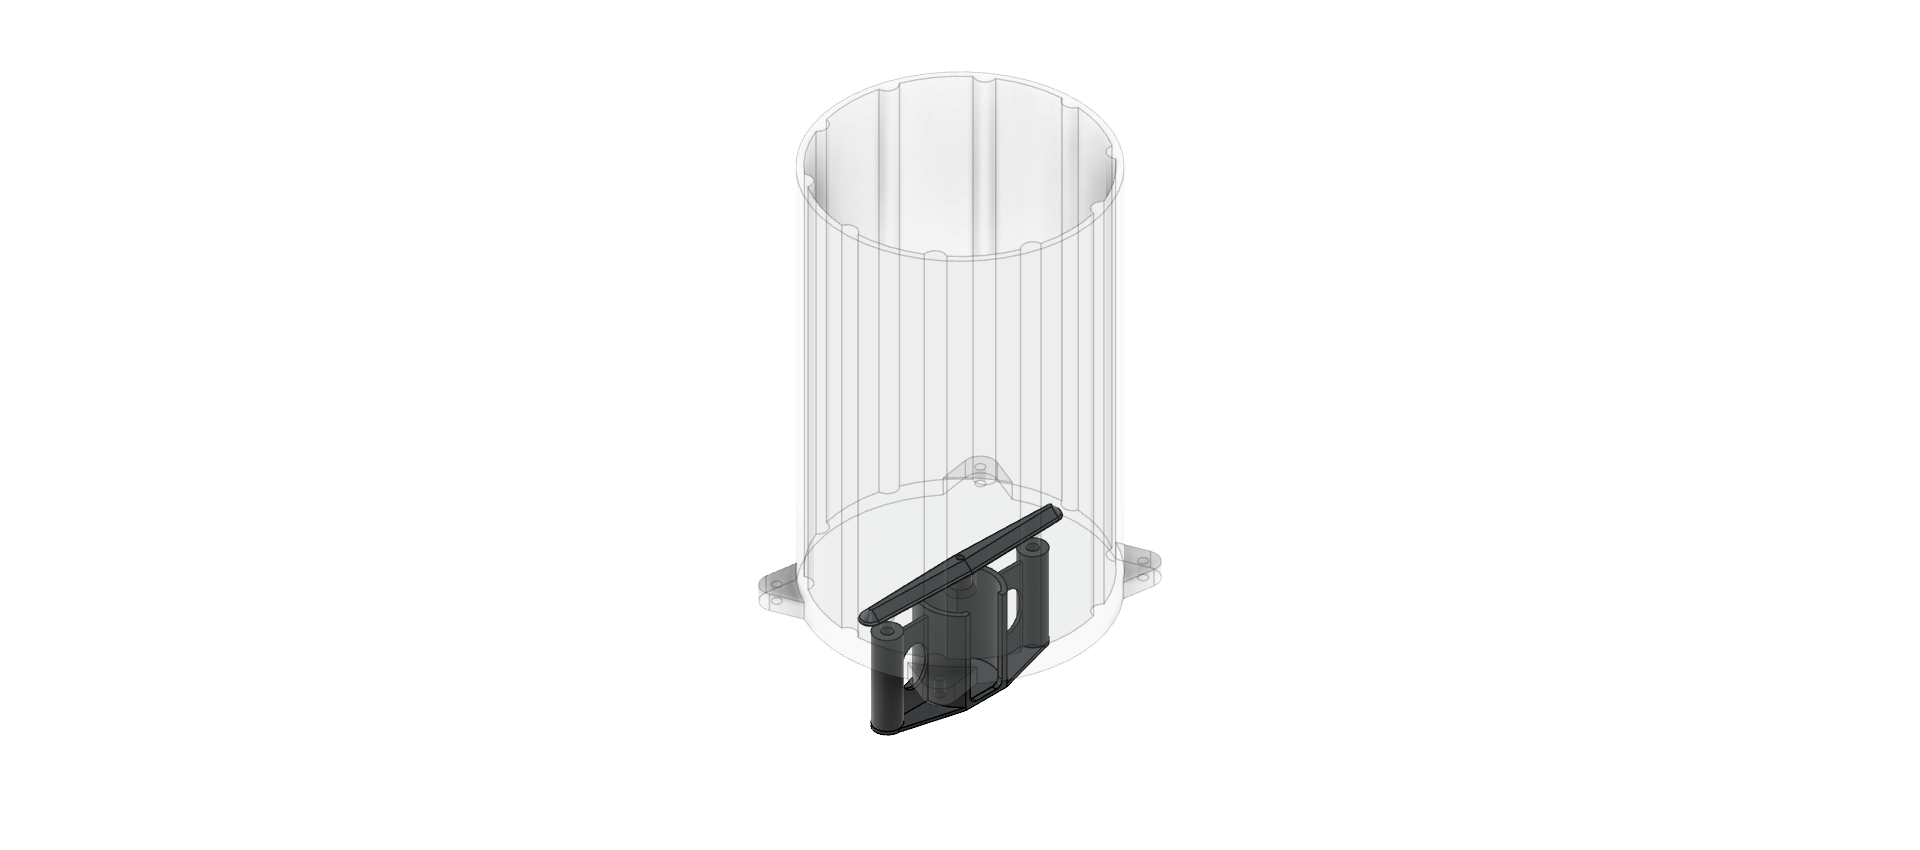
\includegraphics[width=\linewidth]{chapters/03-praca-wlasna/figures/uchwyt_v1.png}
        \caption{\label{fig:uchwyt_v1}Pierwsza wersja uchwytu silnika oraz śmigło względem kubka.}
    \end{minipage}
    \hfill
    \begin{minipage}{0.48\textwidth}
        \centering
        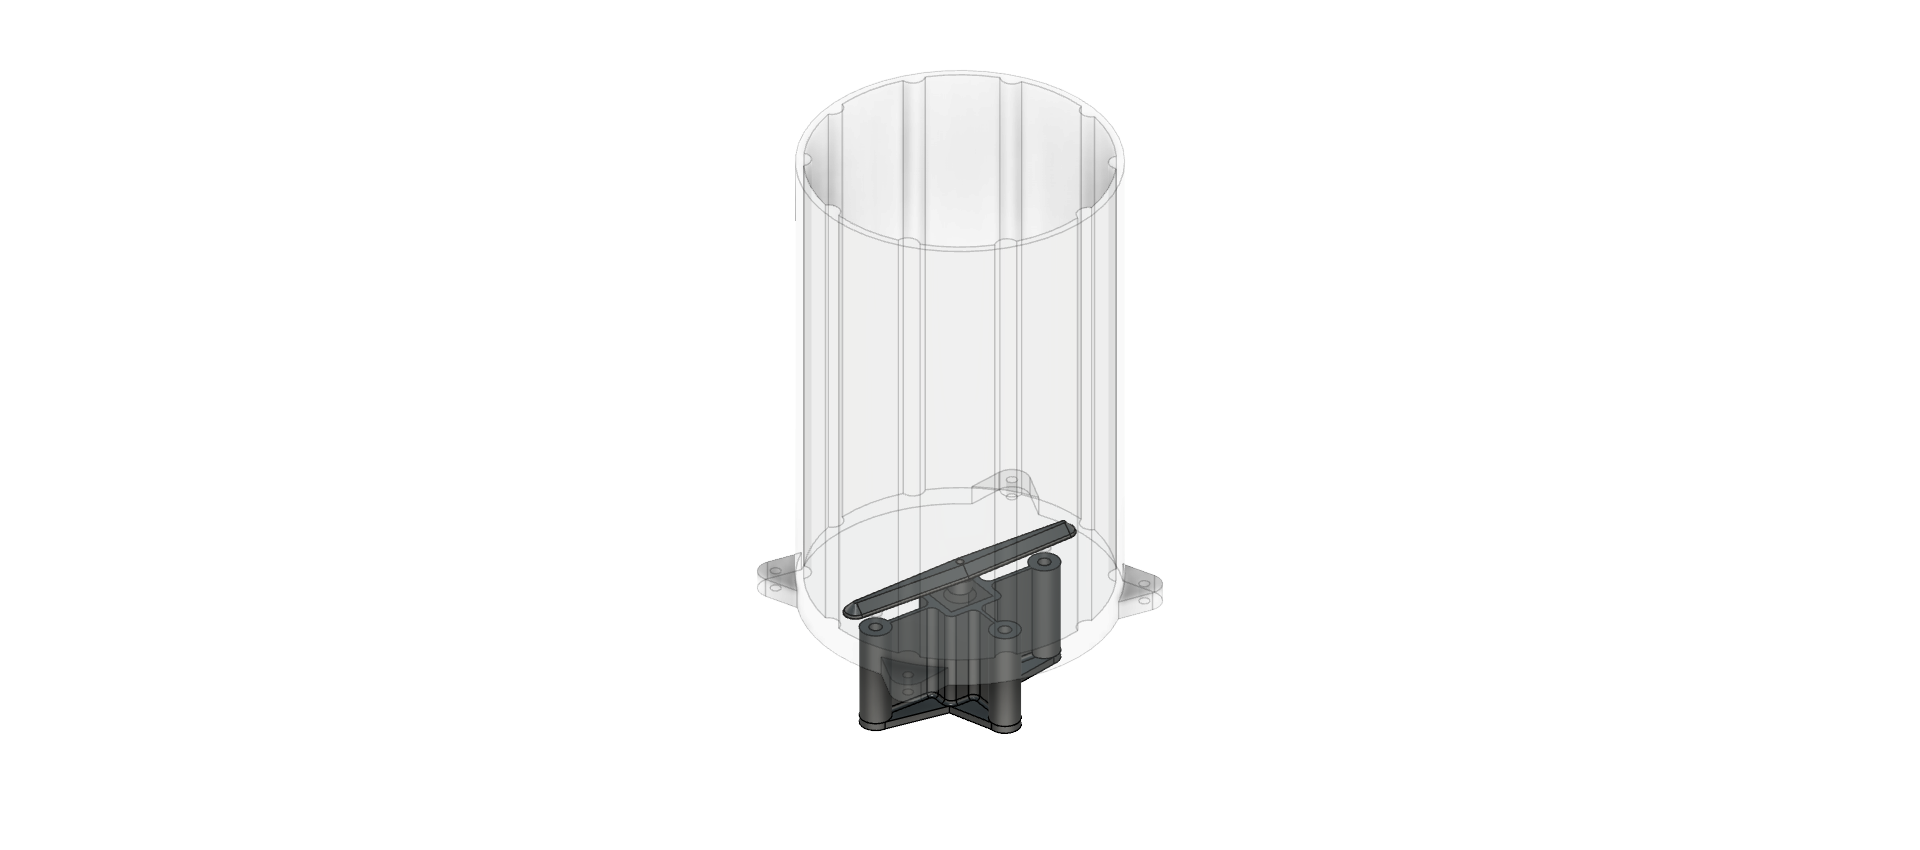
\includegraphics[width=\linewidth]{chapters/03-praca-wlasna/figures/uchwyt_v2.png}
        \caption{\label{fig:uchwyt_v2}Druga wersja uchwytu silnika oraz śmigło względem kubka.}
    \end{minipage}
\end{figure}


Do mocowania Raspberry Pi zaprojektowano specjalną płykę przykręcaną do boku obudowy, którą przedstawiono na Rys.\ref{fig:mainboard}. W projekcie tej płytki uwzględniono otwory do przymocowania Raspberry
Pi oraz układu ULN2803A Darlington. Dodatkowo przygotowano specjalne miejsce do mocowania przycisku. Na płytnce pozostawiono również miejsce
na zamontowanie szyny zasilania. Płytkę tą umieszczono w obudowie w taki sposób, żeby znajdowała się ona bezpośrednio nad wentylatorem. Dzięki temu
strumień powietrza bezpośrednio chłodzi najważniejsze elementy elektroniczne robota. Przycisk zamocowano na tej samej płytce, z wykorzystaniem
dodatkowego elementu wydukowanego na drukarce 3D. Dzięki temu znalazł się on bezpośrednio przy ściance obudowy, a dodatkowo jego mocowanie
nadal spełnia założenie modułowości poprzez mocowanie za pomocą śrub i insertów.

\begin{figure}[H]
    \centering
    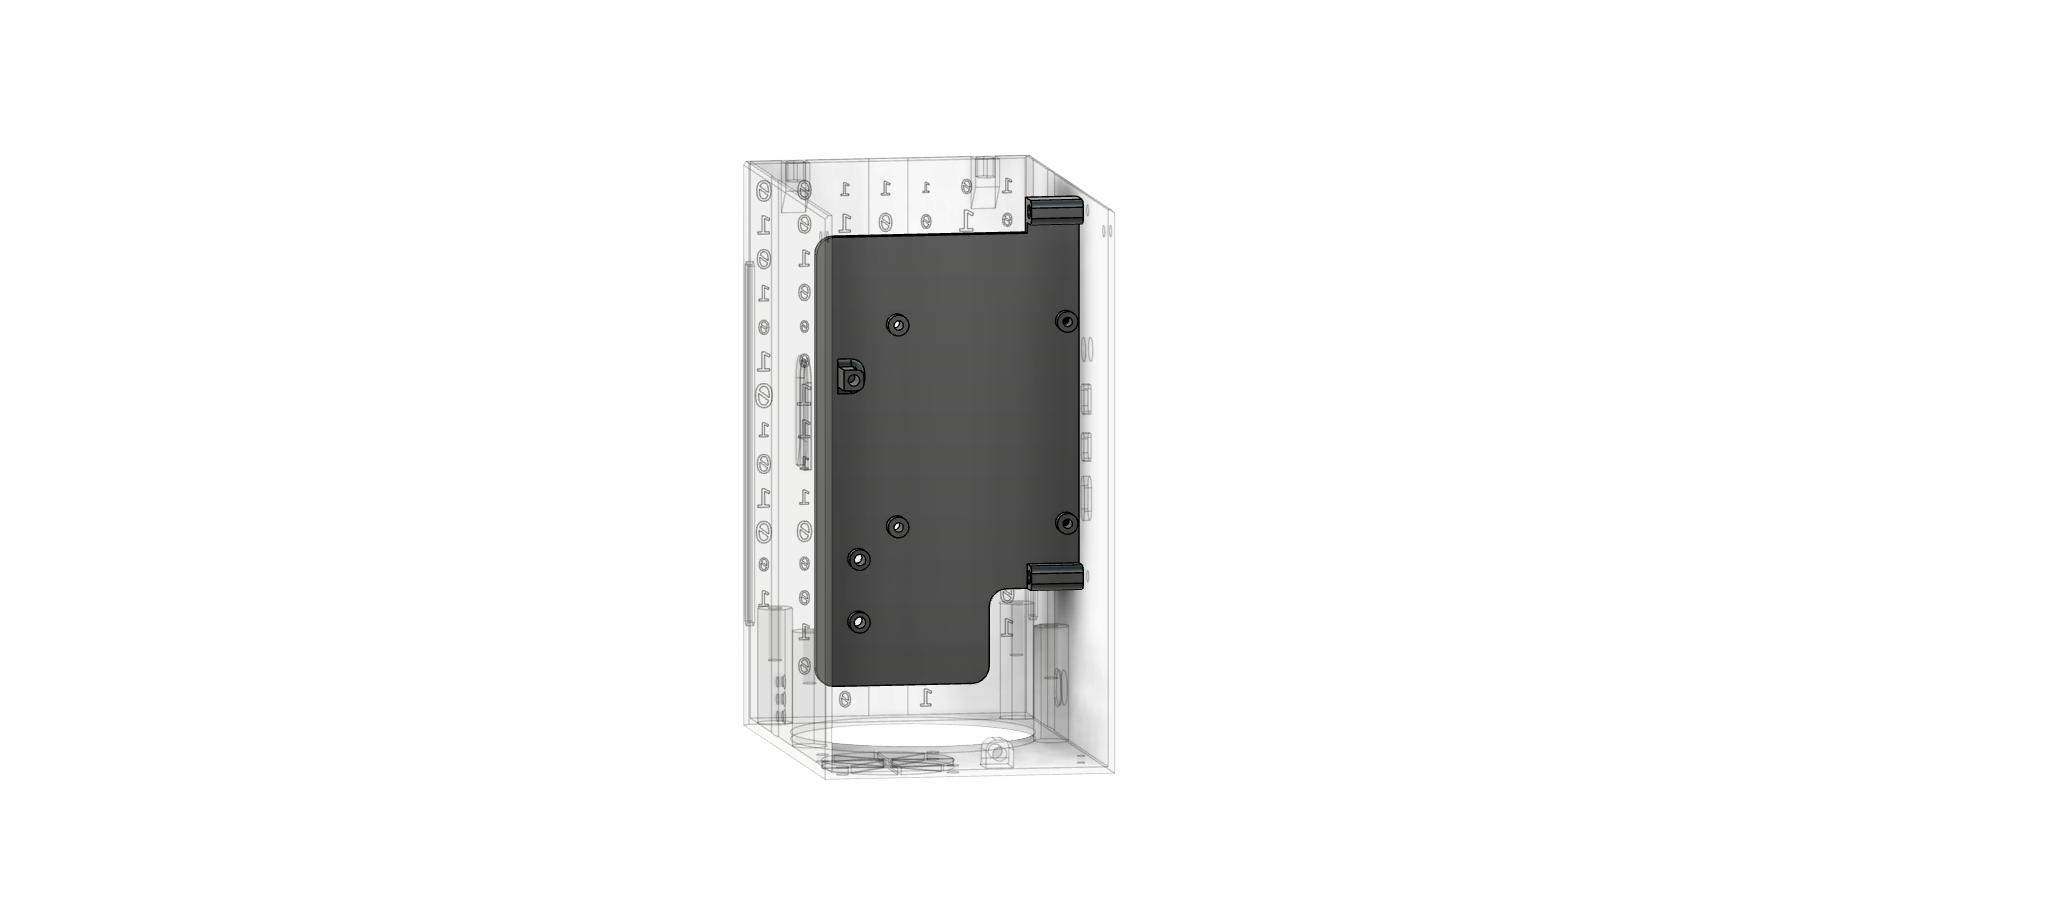
\includegraphics[width=0.95\linewidth]{chapters/03-praca-wlasna/figures/main_board.png}
    \caption{\label{fig:mainboard}Płytka do montażu elektroniki.}
\end{figure}

Układ sterujący silnikiem L298 przykręcono do obudowy pośrednio, poprzez specjalnie zaprojektowane i wydrukowane mocowanie. Dzięki temu wykorzystano
gotowe otwory na śruby znajdujące się w płytce układu L298. Na Rys.\ref{fig:steownik}, na którym przedstawiono płytkę do mocowania elektroniki
z zamontowaną Raspberry Pi 4b oraz układ L298 wiczoczne jest wspominane mocowanie służące do przykręcenia układu L298 do dna obudowy robota.

\begin{figure}[H]
    \centering
    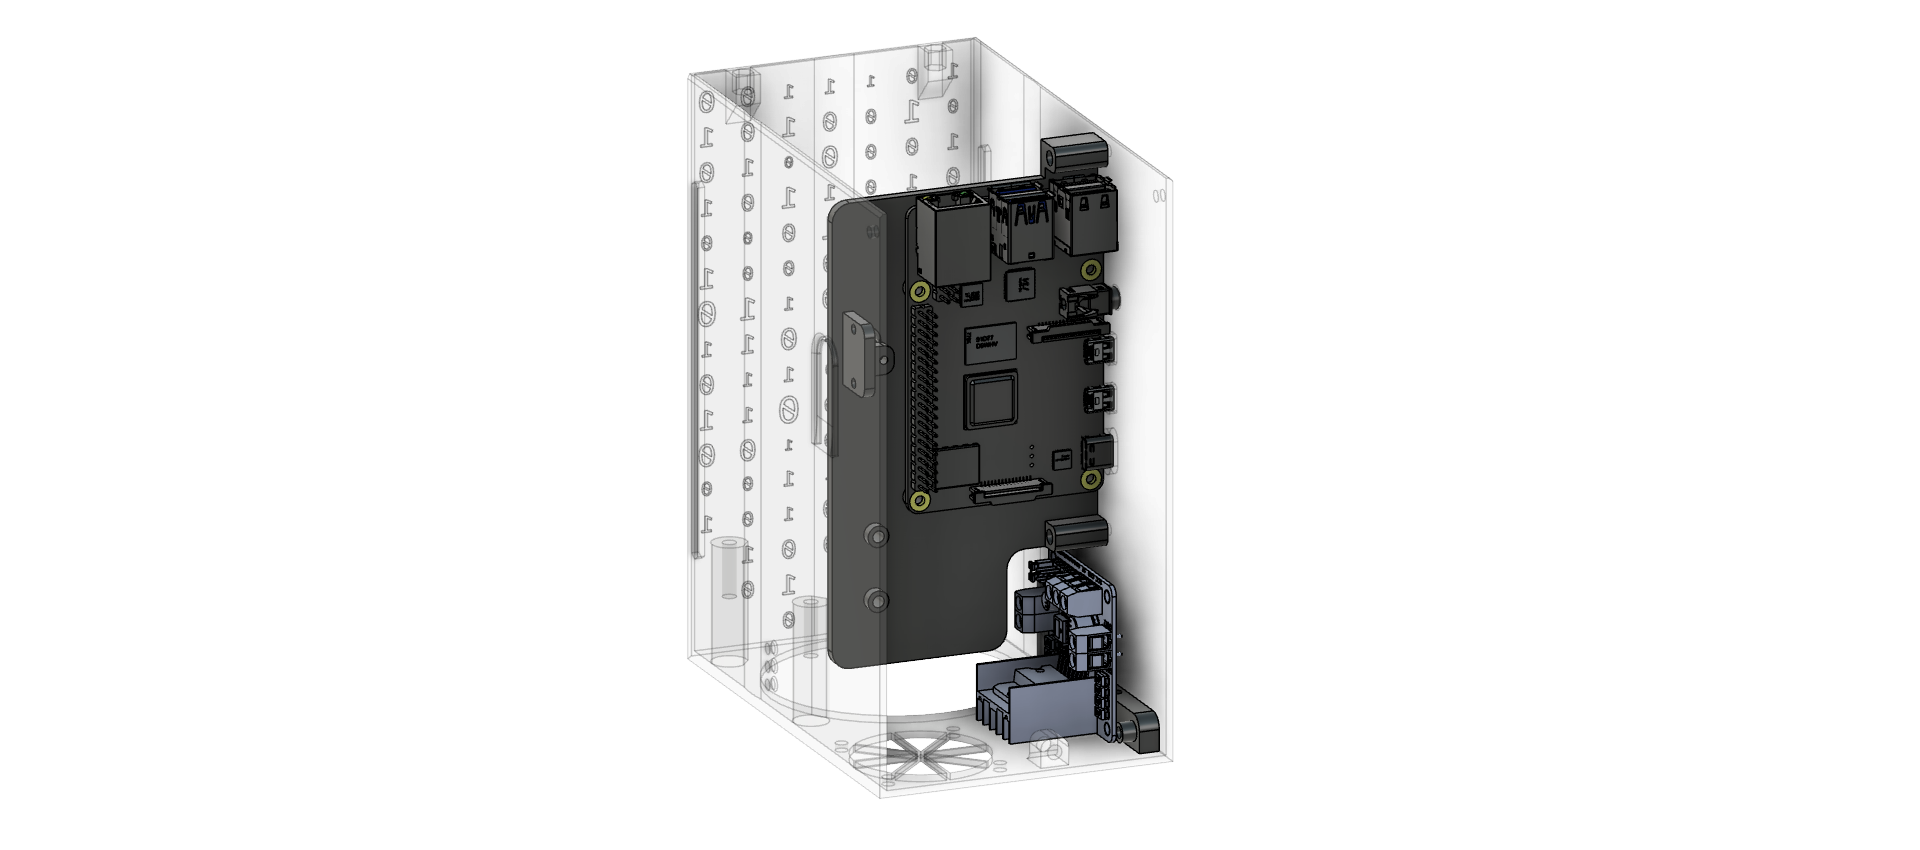
\includegraphics[width=0.95\linewidth]{chapters/03-praca-wlasna/figures/l298n.png}
    \caption{\label{fig:steownik}Zamocowany sterownik L298 z widoczną płytką na której zamocowana jest Raspberry Pi 4b.}
\end{figure}

Do dna obudowy robota przymocowano, za pomocą śrub, również wentylator.

Obudowę zaprojektowano w taki sposób żeby pomieściła wszystkie powyższe elementy. W jej scianach zaprojektowano otwory na wyjścia Raspberry Pi, 
diody LED oraz gniazdo zasilania. W scianie obudowy na wysokości miejsca, w którym znajduje się wewnątrz przycisk, zaprojektowano specjalne wycięcie.
Dzięki dodatkowemu zmniejszeniu grubosci sciana obudowy w tym miejscu jest bardziej elastyczna co pozwala na kliknięcie przycisku znajdującego
się po wewnętrznej stronie ściany obudowy. Na dnie obudowy zaprojektowo również specjalne słupki służące za podpórki dla kubka. 
W słupkach tych zaprojektowano otwory na inserty dzięki, którym kubek można przykręcić do obudowy gwarantując tym jego stabilność.

Podczas projektowania obudowy przewidziano także takie elemementy jak wycięcia od spodu bezpośrednio pod wentylatorem, służące za wlot powietrza 
oraz wycięcia w tylnej ściance, służące za wylot powietrza. Dodatkowo w dnie umieszczono duży utwór możliwiający swobodne mocowanie oraz dostęp do 
silnika, diod LED oraz gniazda zasilania. Na bocznych ścianach zaprojektowano przerwy, które następnie zaślepiono kontrastującym kolorystycznie filamentem.
Przerwy te tak samo jak cyfry na przedniej ścianie obudowy są tylko i wyłącznie elemetami estetycznymi. Ostatnim elementem robota są zaprojektowane nóżki, 
które przyklejono do dna robota. Zapewniają one przepływ powietrza pod robotem gdzie znajduje się wlot powietrza do wentylatora. Gotowy model robota przedstawiono
na Rys.\ref{fig:gotowy}.

\begin{figure}[H]
    \centering
    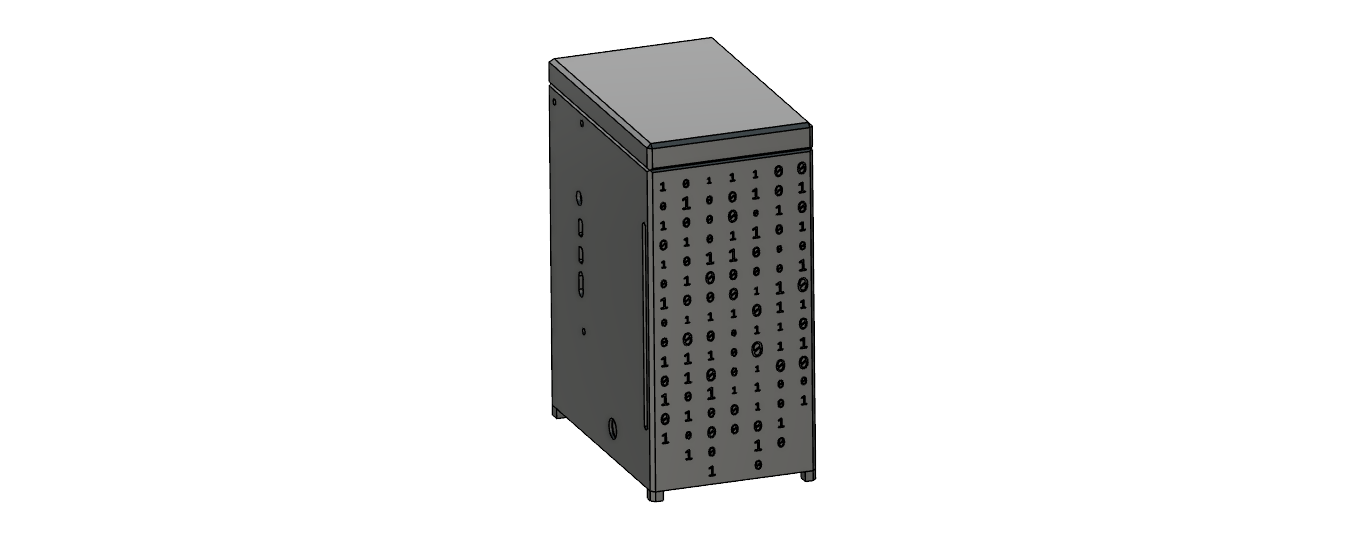
\includegraphics[width=0.95\linewidth]{chapters/03-praca-wlasna/figures/gotowy2.png}
    \caption{\label{fig:gotowy}Projekt gotowego robota od frontu.}
\end{figure}